\documentclass[a4paper, 12pt]{article}
%\usepackage[utf8]{inputenc}
%\usepackage[vietnamese,english]{babel}
\usepackage[utf8]{vietnam}
\usepackage[margin = 2cm]{geometry}
\usepackage{graphicx}
\usepackage{amssymb}
\usepackage{amsthm}
\usepackage{amsmath}
\usepackage{xcolor}
\usepackage{nameref}
\usepackage{babel}
\usepackage{hyperref}
\usepackage[pages=some]{background}
%\usepackage{graphics}
\usepackage{float}
\usepackage{enumerate}
\usepackage[]{enumitem}

\usepackage{multicol}
\usepackage{multirow}
% Set 1.5line spacing for the whole document
\usepackage{setspace}
\usepackage{array}
\onehalfspacing

% Cấu hình header và footer
\usepackage[]{fancyhdr}
\pagestyle{fancy}
\fancyhf{}
\fancyhead[R]{\texttt{LABORATORY 1 \\ MOS TRANSISTOR CHARACTERIZATION}}
\fancyhead[L]{
\includegraphics[width=0.4\linewidth]{sections/pic/bk_name_en.png}}

\fancyfoot[L]{
	
\includegraphics[height=12pt]{sections/pic/logo_DEE.png} \hspace{4pt}
	\textbf{Department of Electronics}\\
	\textit{EE3117/EE4451 – Digital IC Design Laboratory}
}
\fancyfoot[R]{Page|\thepage}
\renewcommand{\headrulewidth}{0.4pt}
\renewcommand{\footrulewidth}{0.4pt}

% Cấu hình background
\backgroundsetup{
	scale=1,
	color=black, 
	opacity=0.4,
	angle=0,
	contents={
		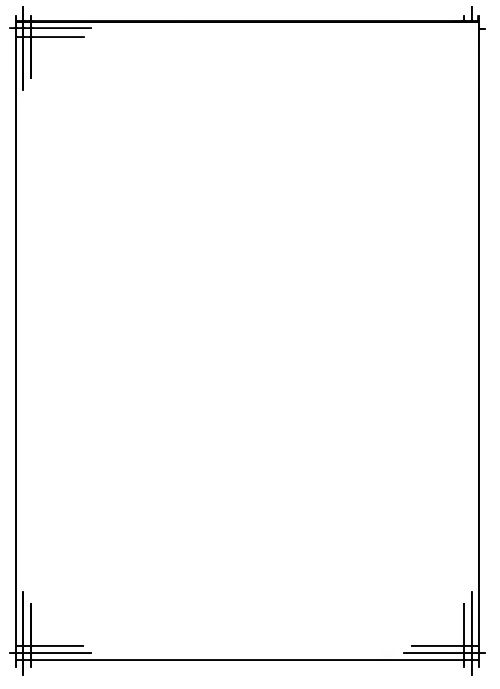
\includegraphics[width=\paperwidth, height=\paperheight]{sections/pic/bia.jpg}
	}
}

% Thêm câu lệnh tạo Item
\newcommand{\itemmini}[1]{%
	\noindent 
\includegraphics[width=0.3cm]{sections/pic/01_logobachkhoatoi.png} #1
}

% Thêm func nhận xét
\newcommand{\comment}[1]{
	\noindent \textbf{Comment:} #1
}

% Thêm func trả lời câu hỏi
\newcounter{questionnumber}
\newenvironment{question}{
	\stepcounter{questionnumber}
	\textbf{Question Experiment \thequestionnumber}
	\begin{enumerate}[leftmargin=*, label = Question \arabic*. ]
	}{
	\end{enumerate}
}

% Môi trường cho câu trả lời
\newenvironment{answer}{
	\vspace{5pt}
	\textbf{Answer:} 
	\begin{itshape}
	}{
	\end{itshape}
	\vspace{10pt}
}

% discussion 
\newenvironment{discussion}{
	\textbf{Discussion}
	\begin{itemize}[label = -]
}{\end{itemize}}
\begin{document}
%	\selectlanguage{vietnamese}
	\BgThispage
\thispagestyle{empty}
\begin{center}
	\Large\textbf{ĐẠI HỌC QUỐC GIA THÀNH PHỐ HỒ CHÍ MINH \\ TRƯỜNG ĐẠI HỌC BÁCH KHOA\\--oo0oo--}
\end{center}
\vspace{0.5cm}
\begin{center}
	
\includegraphics[width=0.3\linewidth]{sections/pic/01_logobachkhoatoi.png}
\end{center}
\vspace{0.4cm}
\begin{center}
	\LARGE\textbf{Digital IC Design Laboratory}
	\vspace{0.1cm}
	
	\Large{LAB 1 - MOS TRANSISTOR CHARACTERIZATION}
\end{center}
\vspace{1cm}

\LARGE

\hspace{2cm}\begin{tabular}{p{0.4\linewidth} p{0.5\linewidth}}
	Giảng viên hướng dẫn: & TS. Trần Hoàng Linh \\
						  & Nguyễn Phan Thiên Phúc \\
%						  & Bùi Lê Quốc Doanh \\
%						  & Phan Tấn Khải \\
\end{tabular}

\vspace{0.5cm}
\begin{center}
	Danh sách thành viên nhóm (47)
	
	\begin{tabular}{|c|p{0.4\linewidth}|p{0.2\linewidth}| c |}
		\hline
		STT & Họ và tên & MSSV & Lớp\\
		\hline
		1 & Hà Phước Việt Quốc & 2212832 & L02\\
		\hline
		2 & Nguyễn Tuệ & 2213812 & L02\\
		\hline
		3 & Nguyễn Đại Đồng & 2210780 & L01\\
		\hline
	\end{tabular}
\end{center}

\vspace{1cm}
\begin{center}
	\fontsize{8pt}{5pt}\selectfont\textbf{Tp.HCM, \dots/\dots/20\dots}
\end{center}

\newpage
\thispagestyle{empty}
\fontsize{13}{14}\selectfont
\tableofcontents
\listoffigures
%	\selectlanguage{english}
	\fontsize{13}{14}\selectfont
	\newpage
\section{Preparations}

\renewcommand{\arraystretch}{1.5} % Tăng khoảng cách dòng cho dễ đọc
\begin{table}[h]
	\centering
	\begin{tabular}{|c|c|c|c|}
		\hline
		\multicolumn{2}{|c|}{\textbf{Conditions}} & \textbf{Equation of Current $I_{D}$} & \textbf{Operation Region} \\
		\hline
		$V_{GS} < V_{Th}$ & $V_{DS}$ & $I_{D} \approx 0$ & Cutoff \\  
		\hline
		$V_{GS} \geq V_{Th}$ & $V_{DS} < V_{GS} - V_{T}$ &  
		$I_{D} = \mu_{n} C_{ox} \frac{W}{L} (V_{GS} - V_{T}) V_{DS} - \frac{1}{2} V_{DS}^{2}$ & Linear \\  
		\hline
		$V_{GS} \geq V_{Th}$ & $V_{DS} \geq V_{GS} - V_{T}$ &  
		$I_{D} = \frac{1}{2} \mu_{n} C_{ox} \frac{W}{L} (V_{GS} - V_{T})^{2}$ & Saturation \\  
		\hline
	\end{tabular}
	\caption{NMOS Regions of Operation}
	\label{tab:nmos_regions}
\end{table}

	\newpage
\section{Experiment - 1: I-V characteristics of MOS transistors}
\subsection{NMOS}
\begin{figure}[H]
	\centering
	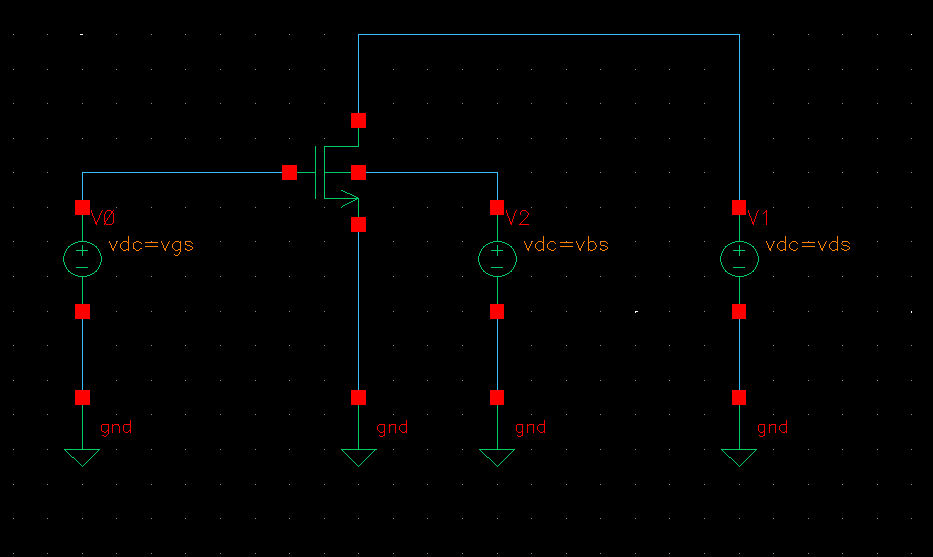
\includegraphics[width = 0.6\linewidth]{sections/pic/EX1_NMOS.png}
	\caption{Test setup for the NMOS\_VTG transistor.}
	\label{f_ex1NMOS-schematic}
\end{figure}

\itemmini{Simulate curves $I_D$ vs $V_{DS}$ @ $V_{GS} = 1V$, and sweeping variable $V_{DS} = [0, 1.5](V)$ step $10mV$.}

\begin{figure}[H]
	\centering
	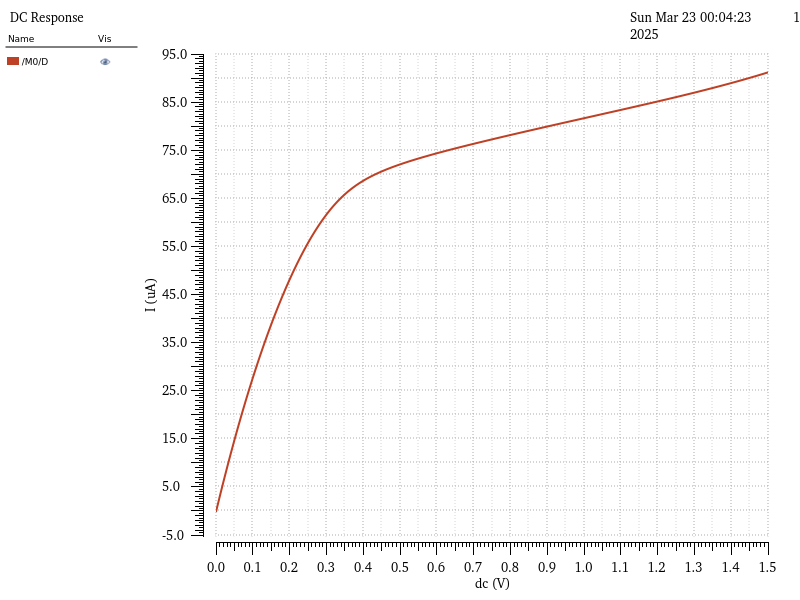
\includegraphics[width=0.6\linewidth]{sections/pic/EX1_NMOS_Id&Vds(Vgs1).png}
	\caption{$I_D$ vs $V_{DS}$ @ $V_{GS} = 1V$, and sweeping variable $V_{DS} = [0, 1.5](V)$ step $10mV$.}
	\label{f_EX1_NMOS_Id&Vds(Vgs1)}
\end{figure}

\begin{discussion}
	\item With \( V_{GS} = 1 \), a conductive channel is formed. Increasing \( V_{DS} \) will increase \( I_{DS} \). For small \( V_{DS} \), \( I_{DS} \) increases linearly, and this region is called the triode region.
	\item When \( V_{DS} \) increases further, entering the saturation region, \( I_{DS} \) does not remain constant as in the ideal model. Instead, it increases slightly due to the channel length modulation effect, which reduces resistance and increases the drain current \( I_{DS} \).
\end{discussion}

\itemmini{Simulate curves $I_D$ vs $V_{GS}$ @ $V_{DS} = 1.5V$, and sweeping variable $V_{GS} = [0, 1.5](V)$ step $10mV$.} 

\begin{figure}[H]
	\centering
	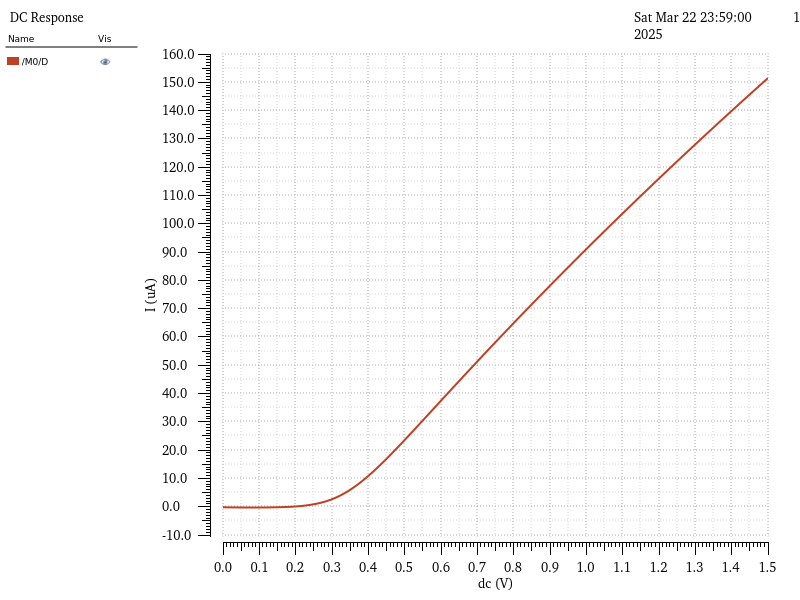
\includegraphics[width=0.6\linewidth]{sections/pic/EX1_NMOS_Id&Vgs(Vds15).png}
	\caption{$I_D$ vs $V_{GS}$ @ $V_{DS} = 1.5V$, and sweeping variable $V_{GS} = [0, 1.5](V)$ step $10mV$.}
	\label{f_EX1_NMOS_Id&Vgs(Vds15)}
\end{figure}

\begin{discussion}
	\item Initially, when \( V_{GS} < V_{TH} \), the NMOS does not form a conductive channel, and the drain-to-source current \( I_{DS} \) is always zero. However, when \( V_{GS} > V_{TH} \), the conductive channel forms, allowing current to flow from the drain to the source. At this point, we can say that the NMOS enters the conduction region.
\end{discussion}

\subsection{PMOS}
\begin{figure}[H]
	\centering
	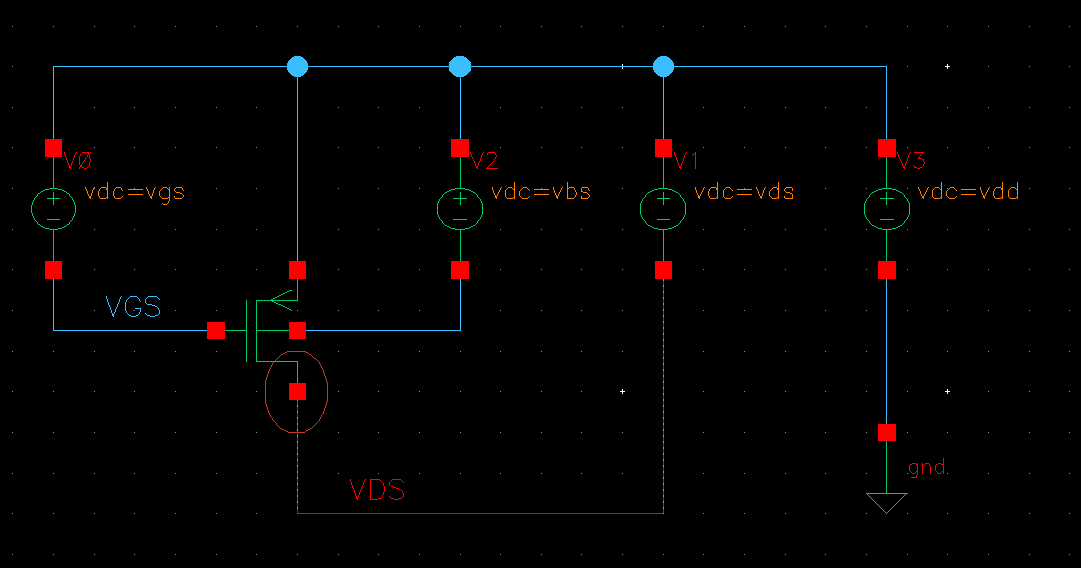
\includegraphics[width = 0.6\linewidth]{sections/pic/EX1_PMOS.png}
	\caption{Test setup for the PMOS\_VTG transistor.}
	\label{f_ex1PMOS-schematic}
\end{figure}

\itemmini{Simulate curves $I_D$ vs $V_{DS}$ @ $V_{SG} = 1V$, and sweeping variable $V_{SD} = [0, 1.5](V)$ step $10mV$.}

\begin{figure}[H]
	\centering
	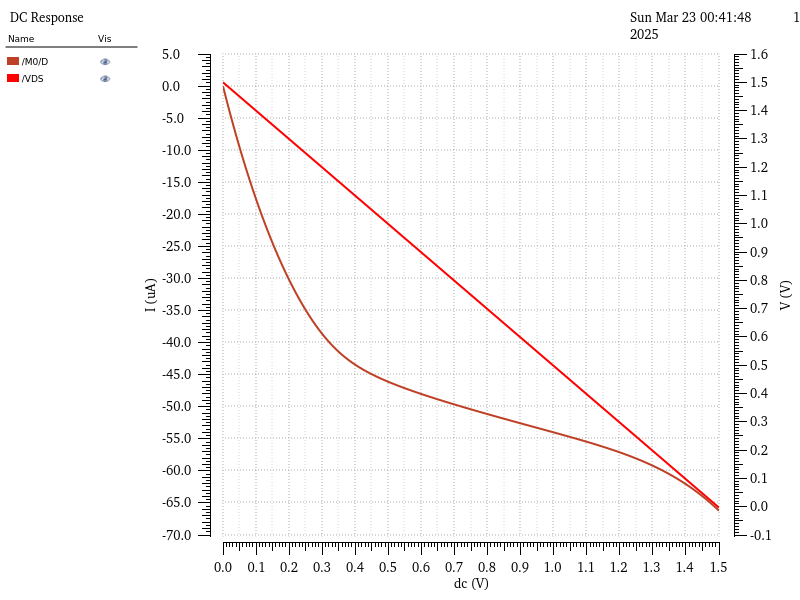
\includegraphics[width=0.6\linewidth]{sections/pic/EX1_PMOS_Id&Vds(Vgs1).png}
	\caption{$I_D$ vs $V_{DS}$ @ $V_{SG} = 1V$, and sweeping variable $V_{SD} = [0, 1.5](V)$ step $10mV$.}
	\label{f_EX1_PMOS_Id&Vds(Vgs1)}
\end{figure}

\itemmini{Simulate curves $I_D$ vs $V_{GS}$ @ $V_{SD} = 1.5V$, and sweeping variable $V_{SG} = [0, 1.5](V)$ step $10mV$.}

\begin{figure}[H]
	\centering
	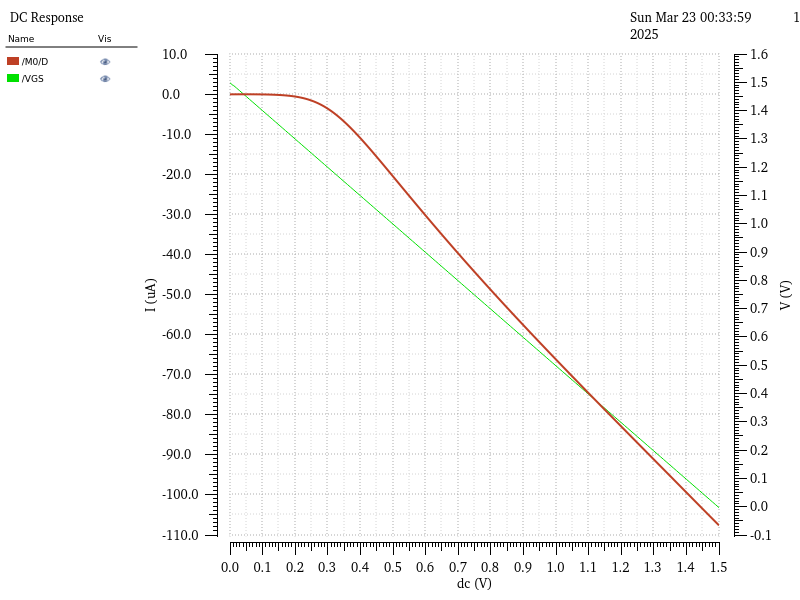
\includegraphics[width=0.6\linewidth]{sections/pic/EX1_PMOS_Id&Vgs(Vds15).png}
	\caption{$I_D$ vs $V_{GS}$ @ $V_{SD} = 1.5V$, and sweeping variable $V_{SG} = [0, 1.5](V)$ step $10mV$.}
	\label{f_EX1_PMOS_Id&Vgs(Vds15)}
\end{figure}

\begin{question}
	\item Based on the $I_D$ vs $V_{GS}$ characteristics, please estimate the threshold voltage $V_{GS}$ of the NMOS transistor. 
	
	\begin{answer}
		In Figure~\ref{f_EX1_NMOS_Id&Vgs(Vds15)}, when \( V_{GS} = 0.28\,\mathrm{V} \), the drain current \( I_{DS} \) begins to increase (deviating from zero). Therefore, the threshold voltage is estimated as \( V_{Th} = 0.28\,\mathrm{V} \) by our group based on the graph.
	\end{answer}
	
	\item Additionally, by analyzing the $I_{D}$ vs $V_{DS}$ characteristics, determine the conduction region of the NMOS transistor when $V_{GS}$ exceeds $V_{Th}$. Specify whether the device operates in the linear (triode) region or the saturation region and provide an explanation.
	
	\begin{answer}
		It is easy to recognize the conduction region of an NMOS transistor when examining the $I_{D}$ versus $V_{GS}$ characteristics. When $V_{GS}$ exceeds $V_{Th}$ (which our group calculated in Question 1), the drain current $I_{DS}$ begins to increase.
		
		$\Rightarrow$ This is the conduction region.
		 		
		The more challenging task is distinguishing between the linear (ohmic) region and the saturation region within the conduction region.
		
		\begin{itemize}[label=-]
			\item The conditions for NMOS operation in the saturation region are:
			\[ 
			V_{GS} > V_{Th} \quad \text{and} \quad V_{DS} \geq V_{GS} - V_{Th}
			\]
			
			\item In the $I_{D}$-$V_{GS}$ characteristics, these conditions are satisfied.
		\end{itemize}
		
		$\Rightarrow$ This represents the saturation region within the conduction region.
	\end{answer}
	
	\item Based on Figure \ref{f_EX1_NMOS_Id&Vds(Vgs1)}, qualitatively determine the operating regions of the NMOS transistor.
	
	\begin{answer}
		\begin{itemize}[label=-]
			\item We see that at $V_{DS} = 0.5V$ the V-I characteristics changing from Triode Region into saturation region.
			
			\item We can calculate the $V_{Th} = V_{GS} - V_{DS} = 0.5(V)$
			
			\item With this result, we can draw operating region table:
			
			\begin{tabular}{|p{0.4\linewidth} | p{0.4\linewidth} |}
				\hline
				Requirements & Operation \\
				\hline
				$V_{GS} < V_{Th} = 0.5$ & Cut off \\
				\hline
				$V_{DS} < V_{GS} - V_{Th} = 0.5$ & Linear \\
				\hline
				$V_{DS} > V_{GS} - V_{Th} = 0.5$ & Saturation\\
				\hline
			\end{tabular} 
		\end{itemize}
	\end{answer}
	
	\item When the NMOS transistor is biased in the saturation region, does the drain current remain constant? Provide a theoretical explanation.
	
	\begin{answer}
		Based on long-channel, ideal, first-order, or Shockley model:
		
		\begin{itemize}[label=-]
			\item At saturation region, based on equation, the drain current remain constant at:
			
			\[ I_{DS} = \dfrac{1}{2} \mu C_{ox} \dfrac{W}{L} (V_{GS} - V_{T})^{2}\]
			
			\item Moreover, with the ideal model we assume that channel-length modulation does not exit, the length of NMOS do not decreasing when $V_{DS}$ increases.
			
		\end{itemize}
		
		$\Rightarrow$ The current $I_{DS}$ do remain in ideal model.
		
		Based on non-ideal model:
		
		\begin{itemize}[label=-]
			\item In non-ideal model, the length of NMOS will decrease when $I_{DS}$ increases leading to the p-n junction between the drain and body forms a depletion region.
			
			\item When the length of the NMOS decreases, it leads to the slightly raising of the current $I_{DS}$ (because resistor value decrease).
			
			\item We have the current equation of $I_{DS}$ in ideal model:
			\begin{align}
				I_{DS} = \dfrac{\beta}{2} V_{GS}^{2} \left(1 + \dfrac{V_{GS}}{V_{A}}\right) \label{eq_EX1_NMOS_ques3}
			\end{align}
		\end{itemize}
		
		$\Rightarrow$ The current $I_{DS}$ do not remain in non-ideal model.
	\end{answer}
	
	\item Propose methods to reduce the slope of the drain current when the NMOS operates in the saturation region. 
	
	\begin{answer}
		\begin{itemize}[label=-]
			\item We increase the length of the NMOS, which reduces the effect of changes in the depletion region between the drain and body on the current, $I_{DS}$.
			\item Based on equation the slope of the current is inverse ratio with L, so L increasing then the current will decrease (Equation \ref{eq_EX1_NMOS_ques3}).
		\end{itemize}
	\end{answer}
\end{question}
	\newpage
\section{Experiment - 2: The effect on IV characteristics when varying $V_{GS}$, and the device's size}
\subsection{NMOS}
\begin{figure}[H]
	\centering
	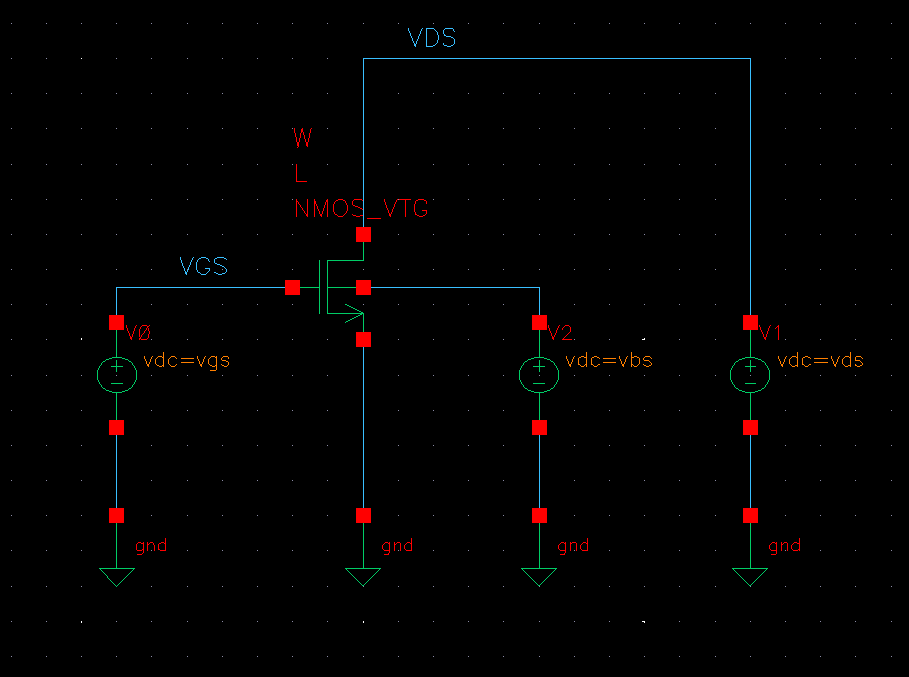
\includegraphics[width = 0.6\linewidth]{sections/pic/EX2_NMOS.png}
	\caption{Testbench NMOS\_VTG for experiment 2.}
	\label{f_ex2NMOS-schematic}
\end{figure}

\itemmini{Simulate curves $I_D$ vs $V_{GS}$ sweeping variable $V_{DS} = [0, 1](V)$ step $0.25V$.}

\begin{figure}[H]
	\centering
	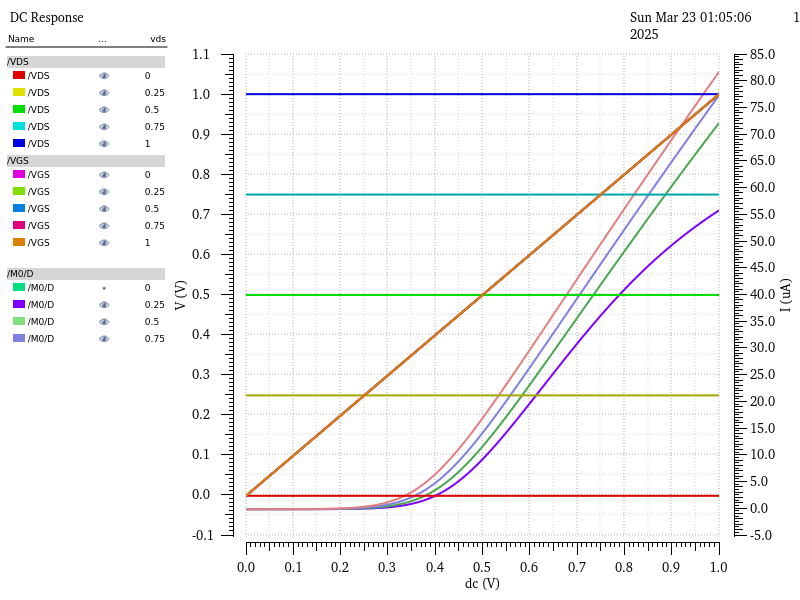
\includegraphics[width = .6\linewidth]{sections/pic/EX2_NMOS_Id&Vgs(Vds_0_1_0_25)(w)(l).png}
	\caption{$I_D$ vs $V_{GS}$ sweeping variable $V_{DS} = [0, 1](V)$ step $0.25V$.}
	\label{f_EX2_NMOS_Id&Vgs(Vds_0_1_0_25)(w)(l)}
\end{figure}

\begin{discussion}
	\item With the characteristics explained above, there is a phenomenon where as \( V_{DS} \) increases, \( V_{th} \) is observed to decrease. This is due to the phenomenon of Drain-Induced Barrier Lowering (DIBL).  
	
	\[ |V_{t} = V_{t0} - \eta V_{DS}| \]
	
	$\Rightarrow \text{The threshold voltage } V_{th} \text{ will begin to decrease as } V_{DS} \text{ increases.}$
	
\end{discussion}

\itemmini{Simulate curves $I_D$ vs $V_{DS}$ sweeping variable $V_{GS} = [0, 1](V)$ step $0.25V$.}

\begin{figure}[H]
	\centering
	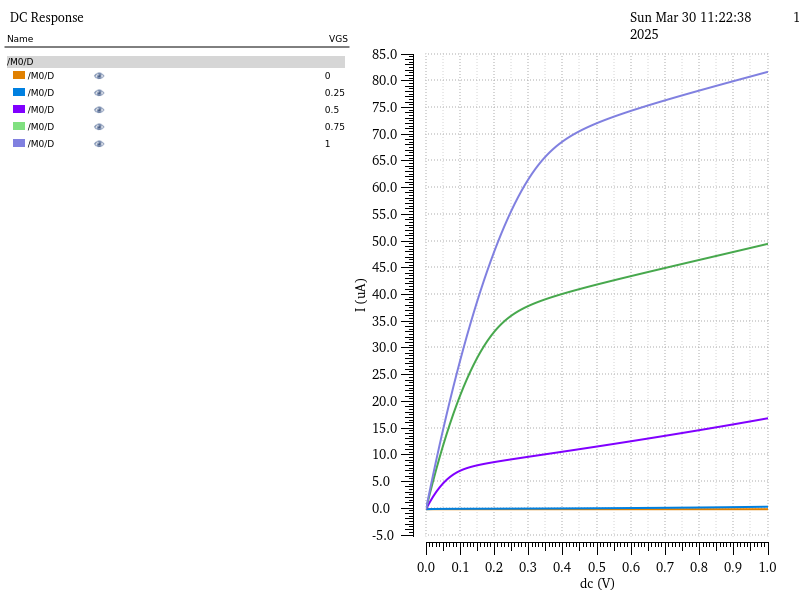
\includegraphics[width = .6\linewidth]{sections/pic/EX2_NMOS_Id&Vds(Vgs_0_1_0_25)(w)(l).png}
	\caption{$I_D$ vs $V_{DS}$ sweeping variable $V_{GS} = [0, 1](V)$ step $0.25V$.}
	\label{f_EX2_NMOS_Id&Vds(Vgs_0_1_0_25)(w)(l)}
\end{figure}

\itemmini{Simulate curves $I_D$ vs $V_{DS}$ sweeping variable $W = [30, 210](nm)$ step $30nm$.}

\begin{figure}[H]
	\centering
	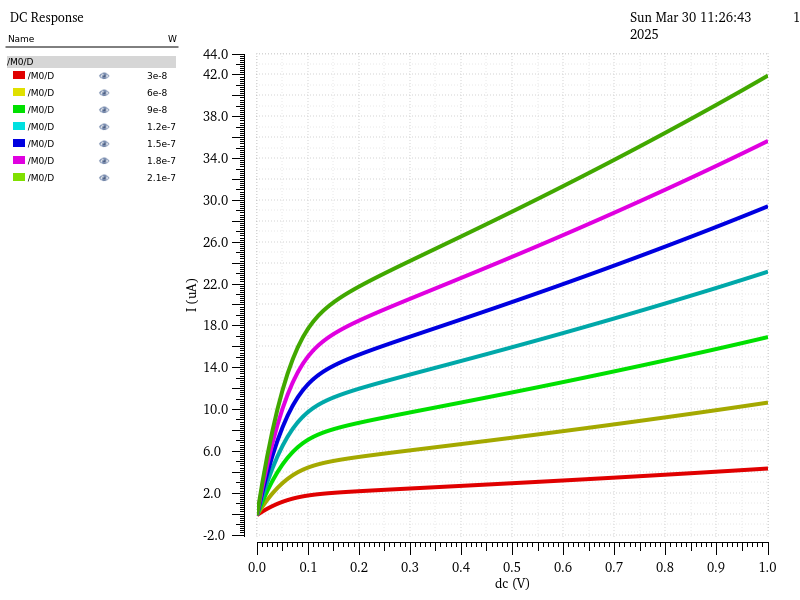
\includegraphics[width = .6\linewidth]{sections/pic/EX2_NMOS_Id&Vds(Vgs(w_30_210)(l).png}
	\caption{$I_D$ vs $V_{DS}$ sweeping variable $W = [30, 210](nm)$ step $30nm$.}
	\label{f_EX2_NMOS_Id&Vds(Vgs(w_30_210)(l)}
\end{figure}

\begin{discussion}
	\item When \( W \) increases, the slope of the \( I_{DS} \) curve in the saturation region also increases. In the figure, we can see that the curves with larger \( W \) have a steeper slope, which aligns with the theory we have learned.  
	
	\item Additionally, we can observe that as \( W \) increases, the resistance decreases, leading to a generally higher \( I_{DS} \) for the same \( V_{DS} \).
	
\end{discussion}

\itemmini{Simulate curves $I_D$ vs $V_{DS}$ sweeping variable $L = [30, 240](nm)$ step $30nm$.}

\begin{figure}[H]
	\centering
	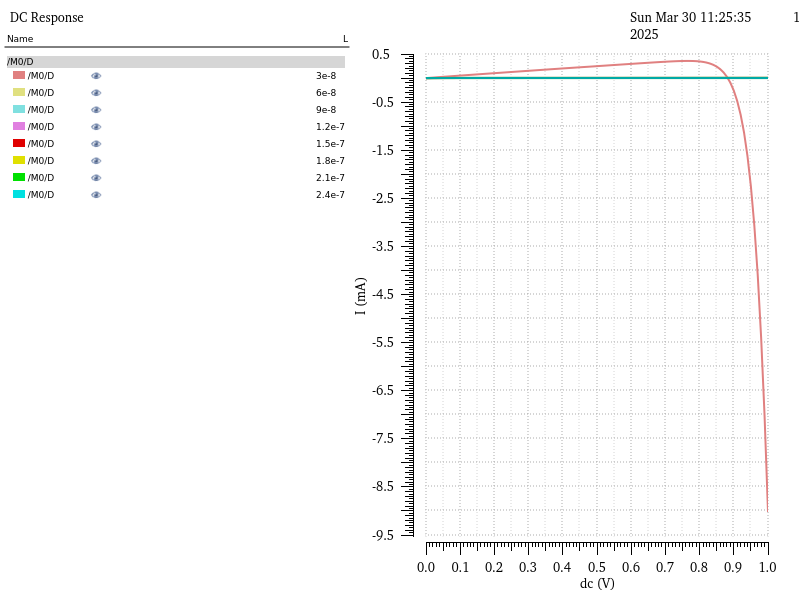
\includegraphics[width = .6\linewidth]{sections/pic/EX2_NMOS_Id&Vds(Vgs(w)(l_30_240).png}
	\caption{$I_D$ vs $V_{DS}$ sweeping variable $L = [30, 240](nm)$ step $30nm$.}
	\label{f_EX2_NMOS_Id&Vds(Vgs(w)(l_30_240)}
\end{figure}

\begin{discussion}
	\item Punch-Through Effect
	\begin{itemize}[label=+]
		\item When \( L \) is too small, the depletion regions from the drain and source can merge, preventing the MOSFET from forming a conductive channel in the usual way.
		\item The electric field from the drain can be strong enough to attract carriers back from the drain to the source, causing the drain current \( I_{D} \) to reverse (negative).
	\end{itemize}
	
	\item Strong DIBL (Drain-Induced Barrier Lowering)
	\begin{itemize}[label=+]
		\item When \( L \) is too small, the drain strongly affects the source region.
		\item The drain voltage can lower the potential barrier at the source, allowing carriers to move from the drain back to the source.
		\item If this effect is strong enough, it can lead to a reversed \( I_{D} \) current.
	\end{itemize}
\end{discussion}

\subsection{PMOS}
\begin{figure}[H]
	\centering
	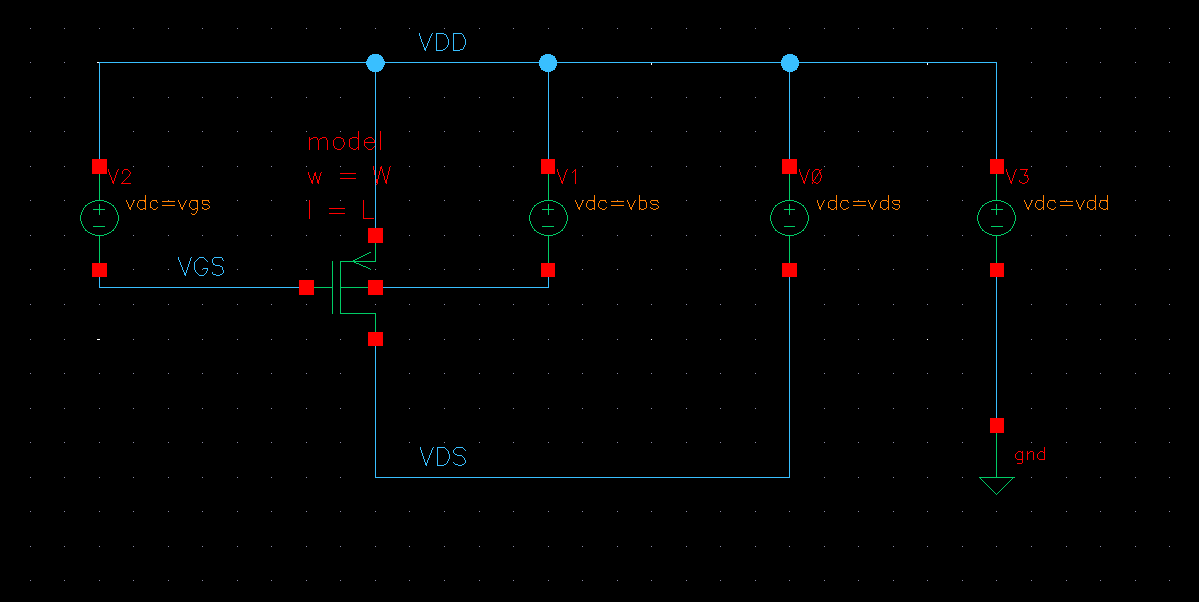
\includegraphics[width = 0.6\linewidth]{sections/pic/EX2_PMOS.png}
	\caption{Testbench PMOS\_VTG for experiment 2.}
	\label{f_ex2PMOS-schematic}
\end{figure}

\itemmini{Simulate curves $I_D$ vs $V_{GS}$ sweeping variable $V_{DS} = [0, 1](V)$ step $0.25V$.}

\begin{figure}[H]
	\centering
	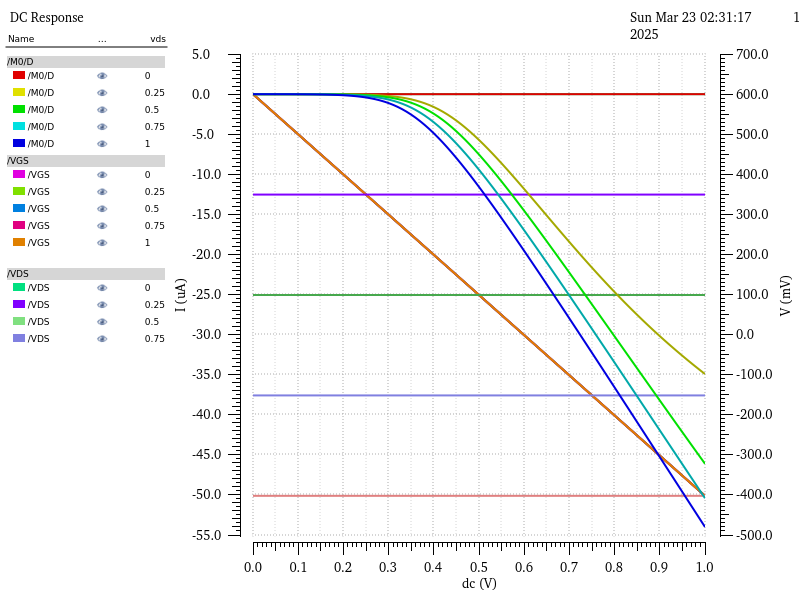
\includegraphics[width = .6\linewidth]{sections/pic/EX2_PMOS_Id&Vgs(Vds_0_1_0_25)(w)(l).png}
	\caption{$I_D$ vs $V_{GS}$ sweeping variable $V_{DS} = [0, 1](V)$ step $0.25V$.}
	\label{f_EX2_PMOS_Id&Vgs(Vds_0_1_0_25)(w)(l)}
\end{figure}

\itemmini{Simulate curves $I_D$ vs $V_{DS}$ sweeping variable $V_{GS} = [0, 1](V)$ step $0.25V$.}

\begin{figure}[H]
	\centering
	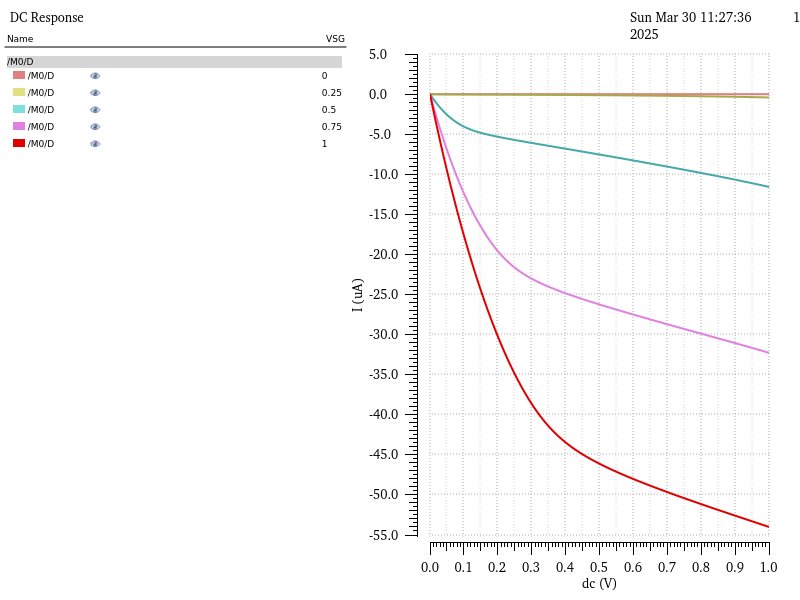
\includegraphics[width = .6\linewidth]{sections/pic/EX2_PMOS_Id&Vds(Vgs_0_1_0_25)(w)(l).png}
	\caption{$I_D$ vs $V_{DS}$ sweeping variable $V_{GS} = [0, 1](V)$ step $0.25V$.}
	\label{f_EX2_PMOS_Id&Vds(Vgs_0_1_0_25)(w)(l)}
\end{figure}

\itemmini{Simulate curves $I_D$ vs $V_{DS}$ sweeping variable $W = [30, 210](nm)$ step $30nm$.}

\begin{figure}[H]
	\centering
	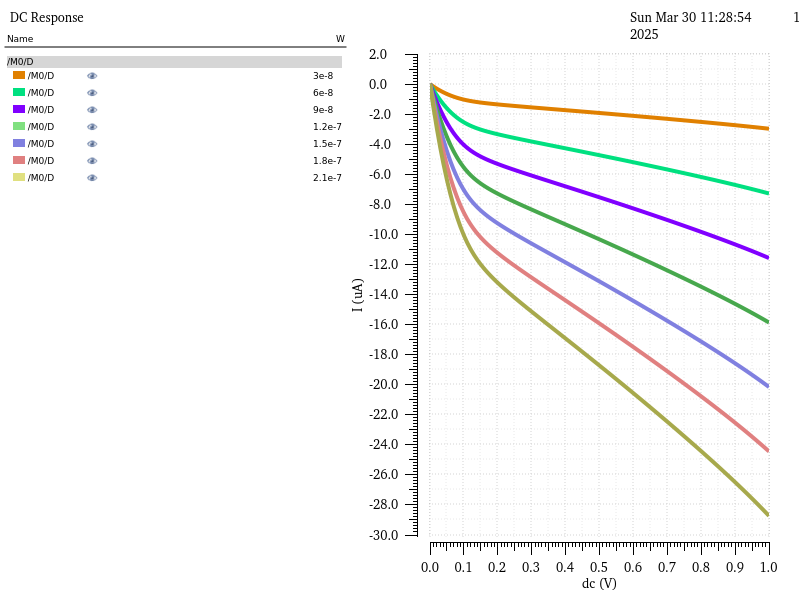
\includegraphics[width = .6\linewidth]{sections/pic/EX2_PMOS_Id&Vds(Vgs(w_30_210)(l).png}
	\caption{$I_D$ vs $V_{DS}$ sweeping variable $W = [30, 210](nm)$ step $30nm$.}
	\label{f_EX2_PMOS_Id&Vds(Vgs(w_30_210)(l)}
\end{figure}

\itemmini{Simulate curves $I_D$ vs $V_{DS}$ sweeping variable $L = [30, 240](nm)$ step $30nm$.}

\begin{figure}[H]
	\centering
	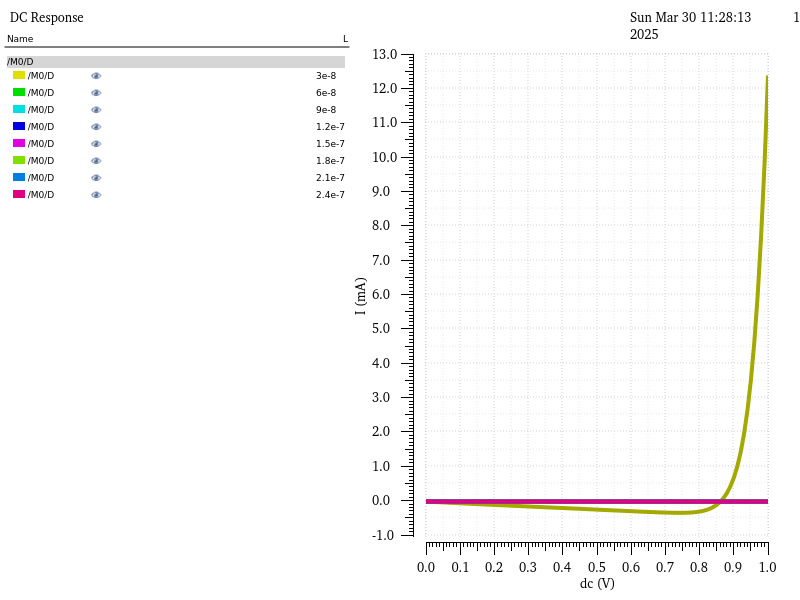
\includegraphics[width = .6\linewidth]{sections/pic/EX2_PMOS_Id&Vds(Vgs(w)(l_30_240).png}
	\caption{$I_D$ vs $V_{DS}$ sweeping variable $L = [30, 240](nm)$ step $30nm$.}
	\label{f_EX2_PMOS_Id&Vds(Vgs(w)(l_30_240)}
\end{figure}
	\newpage
\section{Explore second-order effects (Body effect, Channel-length modulation)}

\subsection{NMOS}

\begin{figure}[H]
	\centering
	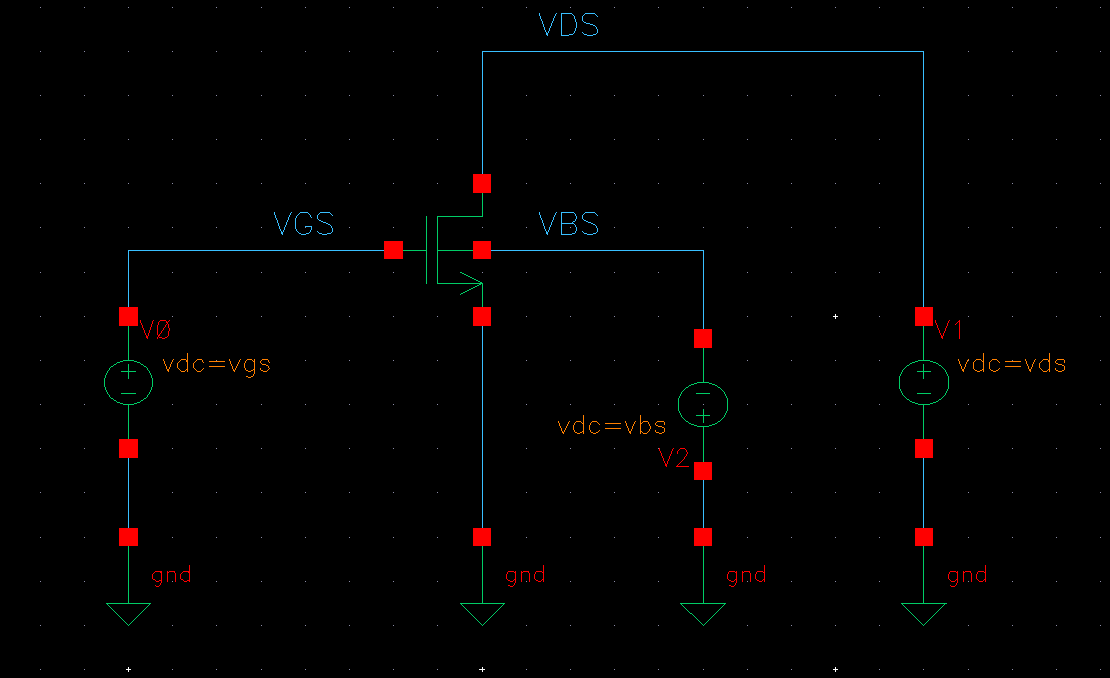
\includegraphics[width = 0.6\linewidth]{sections/pic/EX3_NMOS_schematic.png}
	\caption{Testbench NMOS\_VTG for experiment 3.}
	\label{f_ex3NMOS-schematic}
\end{figure}

\itemmini{Draw curves $I_{D}$ vs $V_{GS}$ @ $V_{DS} = 1V$, $V_{SB} = [0.1, 0.55, 0.9] V$, and sweeping $V_{GS} = [0, 1.5]V$ with step $10mV$.}

\begin{figure}[H]
	\centering
	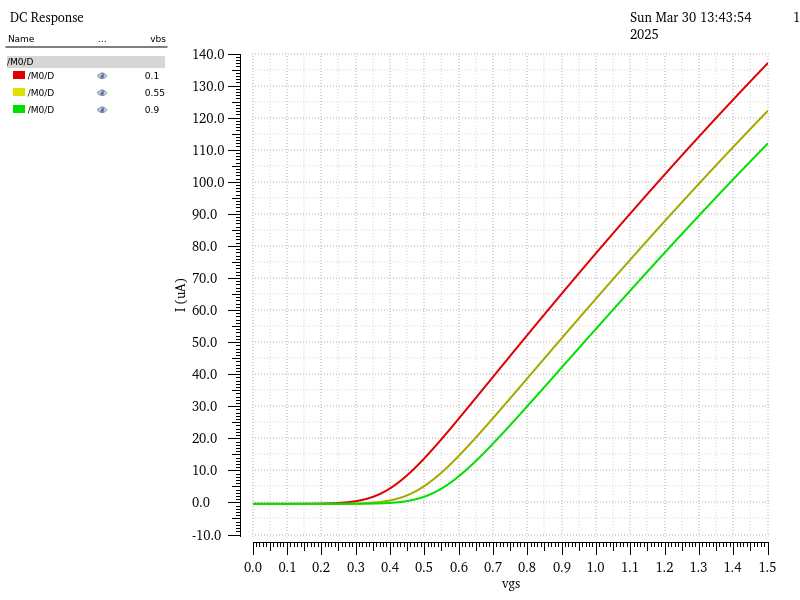
\includegraphics[width=.6\linewidth]{sections/pic/EX3_NMOS_Id&Vgs(Vds=0_1)(w)(l).png}
	\caption{$I_{D}$ vs $V_{GS}$ @ $V_{DS} = 1V$, $V_{SB} = [0.1, 0.55, 0.9] V$, and sweeping $V_{GS} = [0, 1.5]V$ with step $10mV$.}
	\label{f_EX3_NMOS_Id&Vgs(Vds=0_1)(w)(l)}
\end{figure}

\begin{discussion}
	\item When \( V_{SB} \) increases, meaning \( V_{B} \) becomes more negative, the threshold voltage \( V_{TH} \) increases. We can see this phenomenon clearly in the figure. The reason for this is the body effect.  
	
	\[ V_t = V_{t0} + \gamma \left( \sqrt{\phi_{s} + V_{SB}} - \sqrt{\phi_{s}} \right) \]
\end{discussion}

\itemmini{Draw curves $I_{D}$ vs $V_{DS}$ @ $V_{GS} = 1V$, $V_{SB} = [0.1, 0.55, 0.9] V$, and sweeping $V_{DS} = [0, 1.5] V$ with step $10mV$.}

\begin{figure}[H]
	\centering
	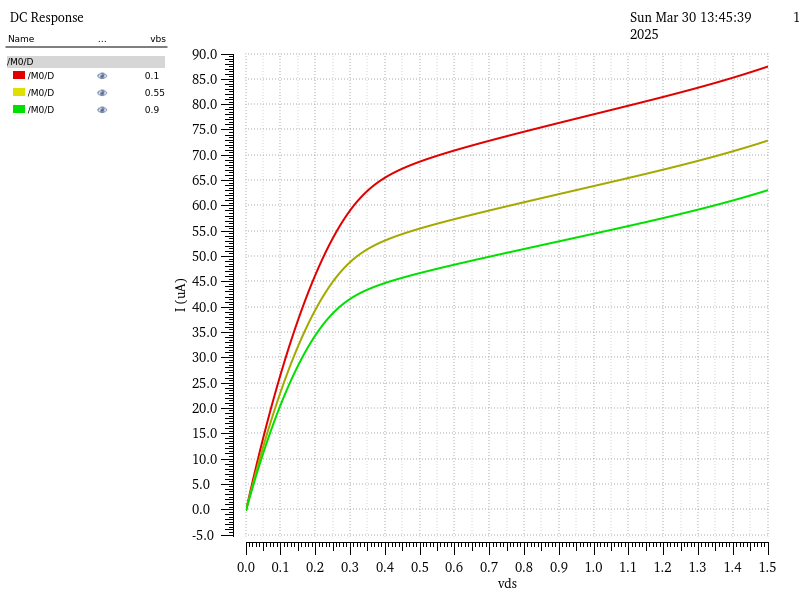
\includegraphics[width=.6\linewidth]{sections/pic/EX3_NMOS_Id&Vds(Vgs=0_1)(w)(l).png}
	\caption{$I_{D}$ vs $V_{DS}$ @ $V_{GS} = 1V$, $V_{SB} = [0.1, 0.55, 0.9] V$, and sweeping $V_{DS} = [0, 1.5] V$ with step $10mV$.}
	\label{f_EX3_NMOS_Id&Vds(Vgs=0_1)(w)(l)}
\end{figure}

\begin{discussion}
	\item With a higher \( V_{TH} \) as \( V_{SB} \) increases, the gate overdrive voltage \( V_{GT} \) becomes smaller. In general, the \( I_{DS} \)-\( V_{DS} \) characteristics tend to be lower and smaller as \( V_{SB} \) increases. 
	
	\[ I_{DS} = \dfrac{\beta}{2} V_{GT}^{2} \left( 1 + \dfrac{V_{DS}}{V_{A}} \right)\]
\end{discussion}

\subsubsection{Measure $\lambda$}
\textbf{Note:} Take points in the saturation region.\\

Draw the curves for $I_{D}$ vs $V_{DS} = [0, 1.5] V$ with a step of $10\text{mV}$, for two values of $V_{GS} = \{0.5, 0.75\} V$ and $V_{BS} = 0V$ for this simulation.\\

\itemmini{For the NMOS transistor with $(Wz/L) = (90n/50n)$.}

\begin{figure}[H]
	\centering
	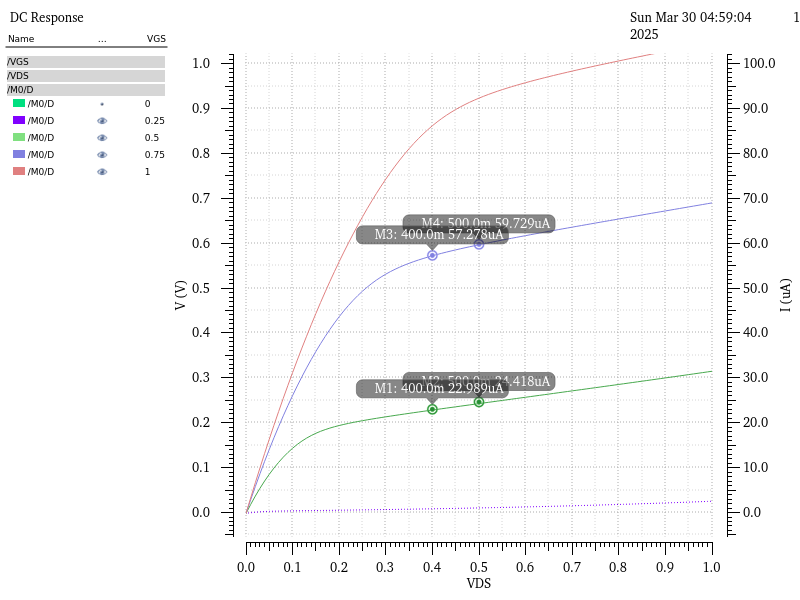
\includegraphics[width=0.6\linewidth]{sections/pic/EX3_NMOS_lambda_(w_l)(90_50).png}
	\caption{$I_{DS}$ vs $V_{DS}$ with a step of $10mV$ for two value of $V_{GS} = \{0.5, 0.75\} V$, the NMOS with $(W/L) = (90n/50n)$}
	\label{f_EX3_NMOS_lambda_(w_l)(90_50)}
\end{figure}

\[ \lambda = \dfrac{I_{D2} - I_{D1}}{I_{D1} V_{DS2} - I_{D2} V_{DS1}} \]

With $V_{GS} = 0.5$, we have:
\[ \lambda = \dfrac{I_{D2} - I_{D1}}{I_{D1} V_{DS2} - I_{D2} V_{DS1}} = \dfrac{(24.42 - 22.99)\times 10^{-6}}{22.99\times 10^{-6}\times 0.5 - 24.42 \times 10^{-6} \times 0.4 }  = 0.82\]

With $V_{GS} = 0.75$, we have:
\[ \lambda = \dfrac{I_{D2} - I_{D1}}{I_{D1} V_{DS2} - I_{D2} V_{DS1}} = \dfrac{(59.73 - 57.28)\times 10^{-6}}{57.28\times 10^{-6}\times 0.5 - 59.73 \times 10^{-6} \times 0.4 }  = 0.52\]

We observe that $\lambda(0.5) > \lambda(0.75)$. This implies that when $V_{GS}$ is low, the stability of $I_{DS}$ in the saturation region is poorer.\\ 

\itemmini{For the NMOS transistor with $(W/L) = (120n/60n)$.}

\begin{figure}[H]
	\centering
	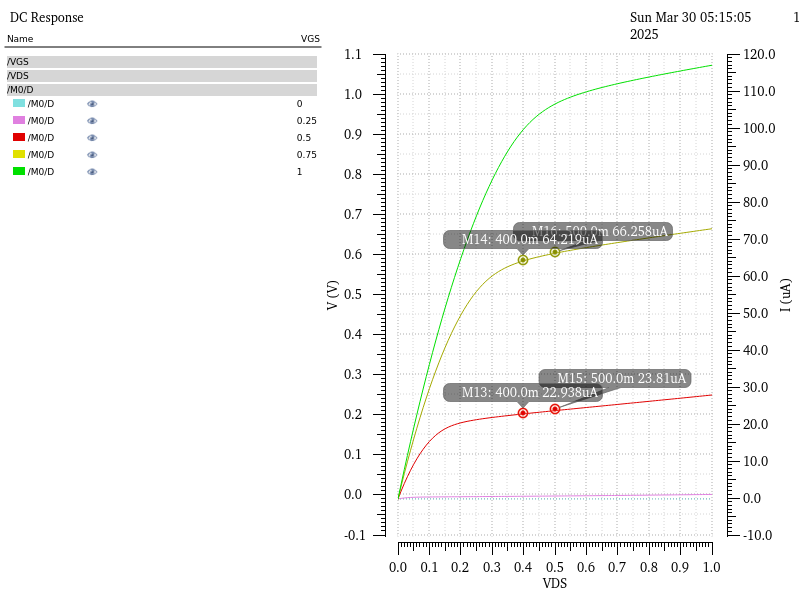
\includegraphics[width=.6\linewidth]{sections/pic/EX3_NMOS_lambda_(w_l)(120_90)(vgs_0_5).png}
	\caption{$I_{DS}$ vs $V_{DS}$ with a step of $10mV$ for two value of $V_{GS} = \{0.5, 0.75\}$, the NMOS with $(W/L) = (120n/60n)$}
	\label{f_EX3_NMOS_lambda_(w_l)(120_90)(vgs_0_5)}
\end{figure}

With $V_{GS} = 0.5$, we have:
\[ \lambda = \dfrac{I_{D2} - I_{D1}}{I_{D1} V_{DS2} - I_{D2} V_{DS1}} = \dfrac{(23.81 - 22.94)\times 10^{-6}}{22.94\times 10^{-6}\times 0.5 - 23.81 \times 10^{-6} \times 0.4 }  = 0.44 \]

With $V_{GS} = 0.75$, we have:
\[ \lambda = \dfrac{I_{D2} - I_{D1}}{I_{D1} V_{DS2} - I_{D2} V_{DS1}} = \dfrac{(66.26 - 64.22)\times 10^{-6}}{64.22 \times 10^{-6}\times 0.5 - 66.25 \times 10^{-6} \times 0.4 }  = 0.37 \]

Thus, for NMOS transistors with smaller technologies, $\lambda$ increases. This is because, as $L$ decreases, the \textit{Short Channel Effect (SCE)} becomes more pronounced, enhancing the dependence of $I_{DS}$ on $V_{DS}$. Consequently, the channel length modulation factor $\lambda$ increases, indicating reduced stability of $I_{DS}$.

\itemmini{Usingtool}
\begin{figure}[H]
	\centering
	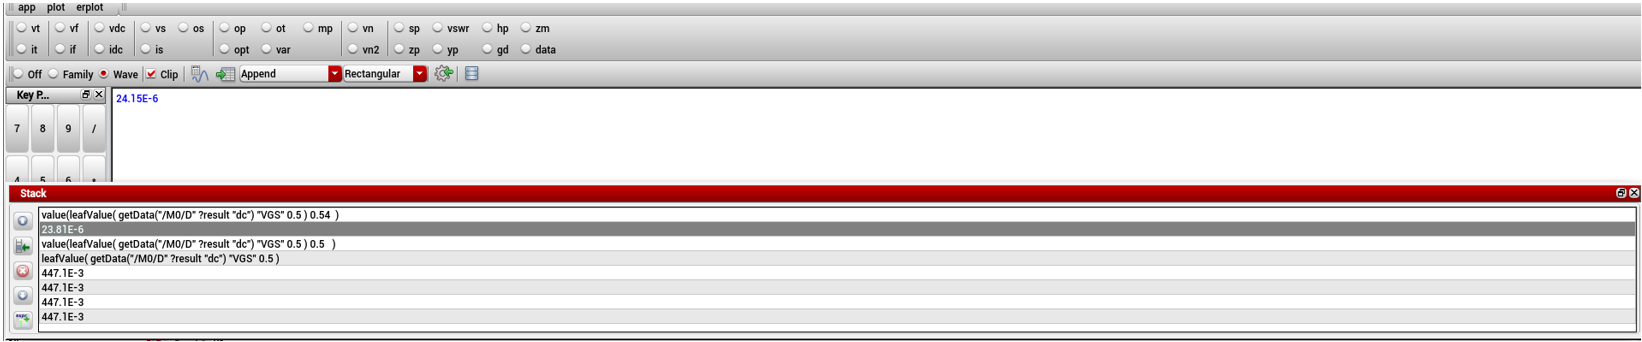
\includegraphics[width=0.8\linewidth]{sections/pic/EX3_NMOS_tool_cal_lambda.png}
	\caption{Use a tool to calculate $\lambda$.}
	\label{f_EX3_NMOS_tool_cal}
\end{figure}

\subsubsection{Measure $V_{Th0}$}
\[ V_{Th} = \dfrac{V_{GS1} - V_{GS2}\sqrt{\dfrac{I_{DS1}}{I_{DS2}}}}{1 - \sqrt{\dfrac{I_{DS1}}{I_{DS2}}}} \]

\itemmini{For the NMOS transistor with $(W/L) = (90n/50n)$.}

\begin{figure}[H]
	\centering
	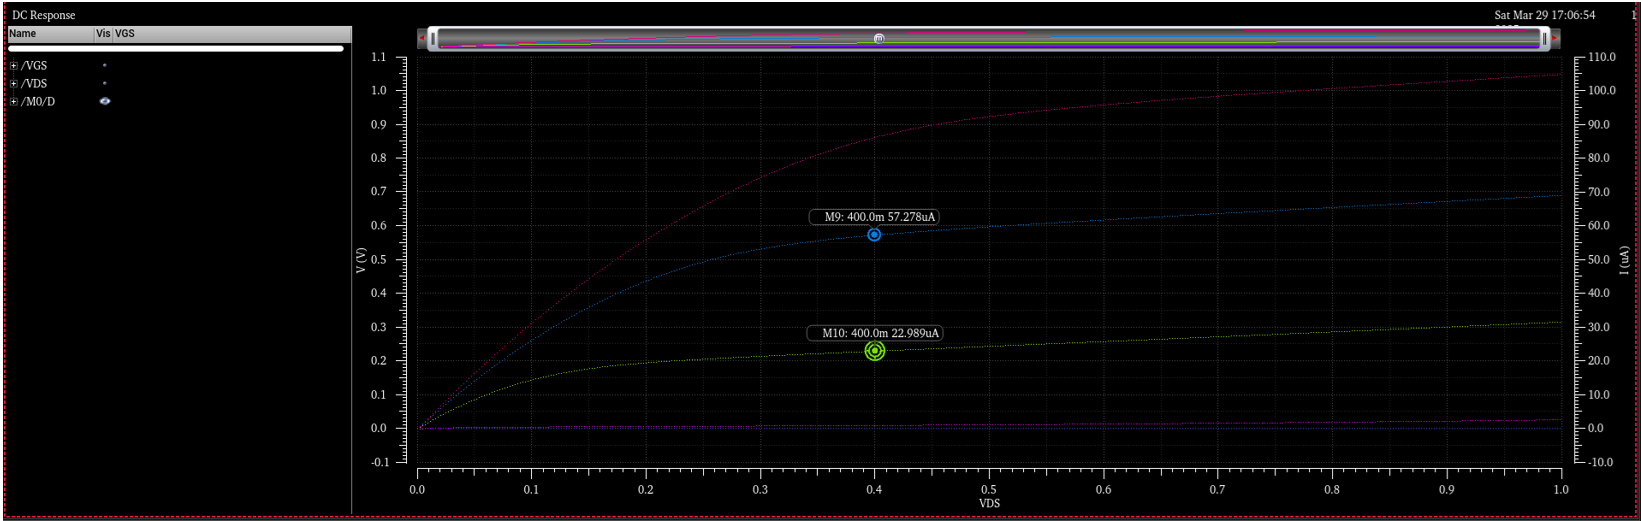
\includegraphics[width=.6\linewidth]{sections/pic/EX3_NMOS_vth0_(w_l)(90_50).png}
	\caption{$I_{DS}$ vs $V_{DS}$ with step $10mV$ with $(W/L) = (90n/50n)$}
	\label{f_EX3_NMOS_vth0_(w_l)(90_50)}
\end{figure}

\[ V_{Th0} = \dfrac{V_{GS1} - V_{GS2}\sqrt{\dfrac{I_{DS1}}{I_{DS2}}}}{1 - \sqrt{\dfrac{I_{DS1}}{I_{DS2}}}} = \dfrac{0.75 - 0.5\times \sqrt{\dfrac{57.28\times 10^{-6}}{22.99\times 10^{-6}}}}{1 - \sqrt{\dfrac{57.28\times 10^{-6}}{22.99\times 10^{-6}}}} = 0.07(V)\]

\itemmini{For the NMOS transistor with $(W/L) = (120n/60n)$.}

\begin{figure}[H]
	\centering
	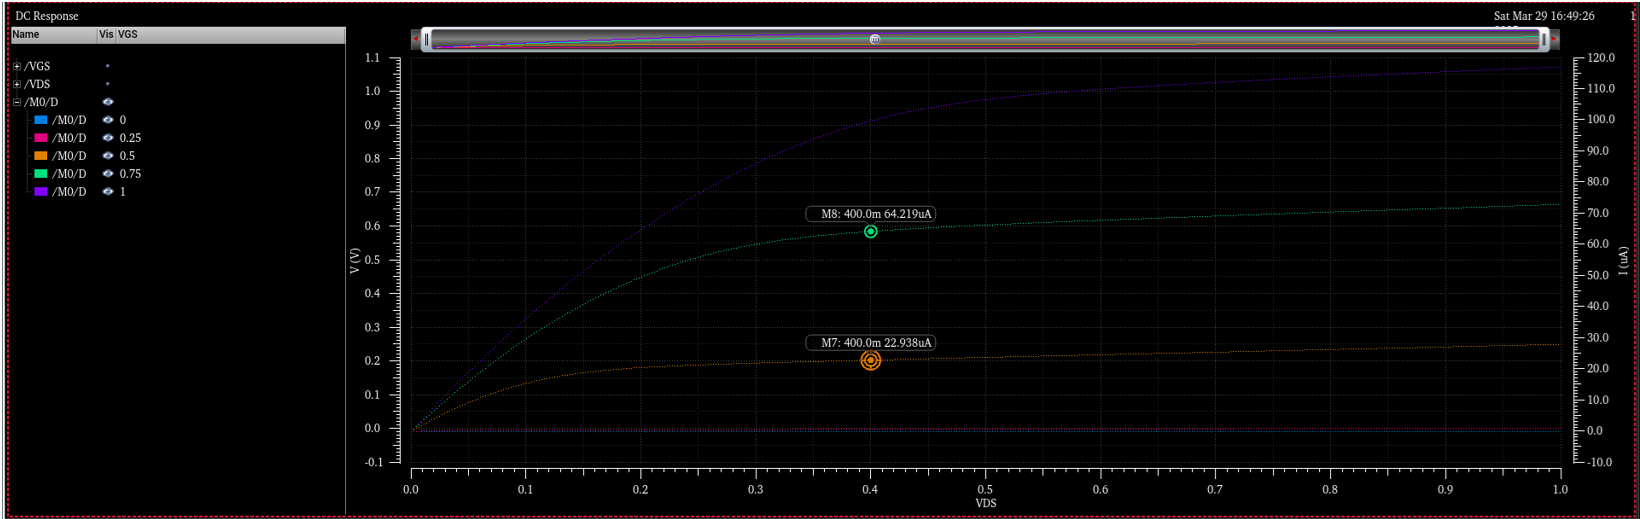
\includegraphics[width=.6\linewidth]{sections/pic/EX3_NMOS_vth0_(w_l)(120_60).png}
	\caption{$I_{DS}$ vs $V_{DS}$ with step $10mV$ with $(W/L) = (120n/60n)$}
	\label{f_EX3_NMOS_vth0_(w_l)(120_60)}
\end{figure}

\[ V_{Th0} = \dfrac{V_{GS1} - V_{GS2}\sqrt{\dfrac{I_{DS1}}{I_{DS2}}}}{1 - \sqrt{\dfrac{I_{DS1}}{I_{DS2}}}} = \dfrac{0.75 - 0.5\times \sqrt{\dfrac{64.22\times 10^{-6}}{22.94\times 10^{-6}}}}{1 - \sqrt{\dfrac{64.22\times 10^{-6}}{22.94\times 10^{-6}}}} = 0.13(V)\] 


When the $W/L$ ratio changes, $V_{TH}$ can be affected due to the \textit{SCE - Short Channel Effect}.

When $L$ decreases (in the case of NMOS $90n/50n$), $V_{TH}$ tends to decrease due to the \textit{Drain-Induced Barrier Lowering (DIBL)} effect.

When $L$ increases (in the case of NMOS $120/60n$), $V_{TH}$ is higher because the short channel effect becomes less pronounced.

\subsubsection{Measure $\gamma$}

\itemmini{For the NMOS transistor with $(W/L) = (90n/50n)$ and $V_{BS} = 0.5$.}

\begin{figure}[H]
	\centering
	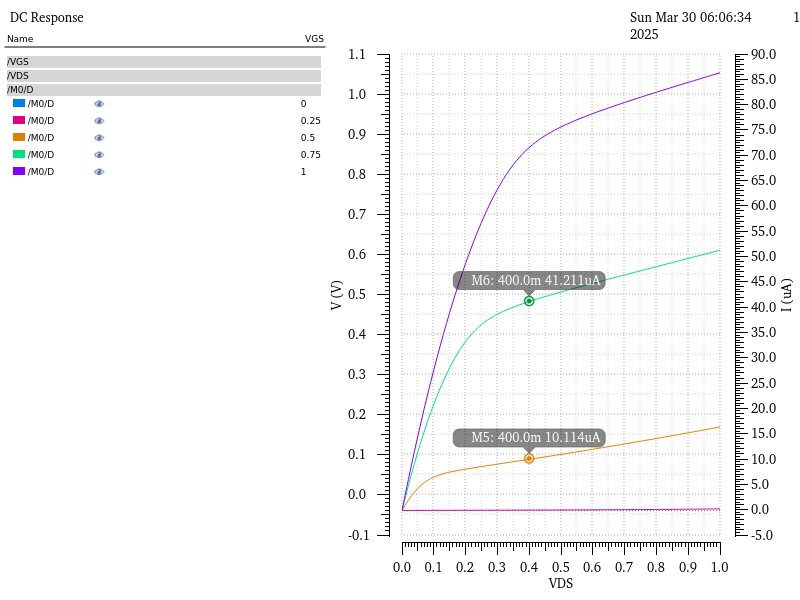
\includegraphics[width=.6\linewidth]{sections/pic/EX3_NMOS_gamma_(w_l)(90_50).png}
	\caption{$I_{DS}$ vs $V_{DS}$ with step $10mV$ with $(W/L) = (90n/50n)$}
	\label{f_EX3_NMOS_gamma_(w_l)(90_50)}
\end{figure}

\[ V_{Th} = \dfrac{V_{GS1} - V_{GS2}\sqrt{\dfrac{I_{DS1}}{I_{DS2}}}}{1 - \sqrt{\dfrac{I_{DS1}}{I_{DS2}}}} = \dfrac{0.75 - 0.5\times \sqrt{\dfrac{41.21\times 10^{-6}}{10.11\times 10^{-6}}}}{1 - \sqrt{\dfrac{41.21\times 10^{-6}}{10.11\times 10^{-6}}}} = 0.25(V)\] 


We have, $2\phi F = 0.7 \gamma$:

\[ \gamma = \dfrac{V_{Th} - V_{Th0}}{\sqrt{|2\phi_{F}| + |V_{BS} } - \sqrt{|2\phi_{F}}} = \dfrac{0.25 - 0.07}{\sqrt{0.7 + 0.5} - \sqrt{0.7}} =0.7 \]

Thus, we can conclude that as $\gamma$ increases, $V_{Th}$ rises more significantly compared to when $V_{BS}$ increases.\\

\itemmini{For the NMOS transistor with $(W/L) = (120n/60n)$ and $V_{BS} = 0.5$.}

\begin{figure}[H]
	\centering
	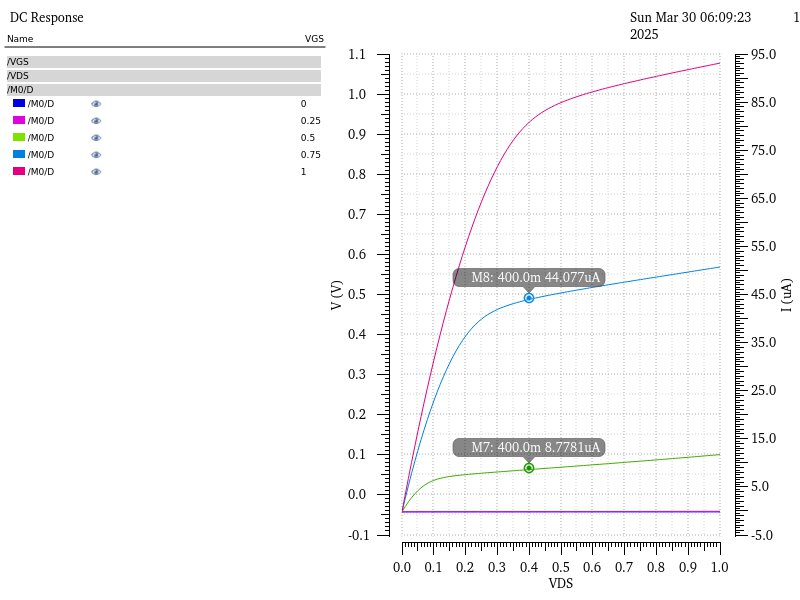
\includegraphics[width=.6\linewidth]{sections/pic/EX3_NMOS_gamma_(w_l)(120_60).png}
	\caption{$I_{DS}$ vs $V_{DS}$ with step $10mV$ with $(W/L) = (120n/60n)$}
	\label{f_EX3_NMOS_gamma_(w_l)(120_60)}
\end{figure}

\[ V_{Th} = \dfrac{V_{GS1} - V_{GS2}\sqrt{\dfrac{I_{DS1}}{I_{DS2}}}}{1 - \sqrt{\dfrac{I_{DS1}}{I_{DS2}}}} = \dfrac{0.75 - 0.5\times \sqrt{\dfrac{44.07\times 10^{-6}}{8.78\times 10^{-6}}}}{1 - \sqrt{\dfrac{44.07\times 10^{-6}}{8.78\times 10^{-6}}}} = 0.3(V)\] 

\[ \gamma = \dfrac{V_{Th} - V_{Th0}}{\sqrt{|2\phi_{F}| + |V_{BS} } - \sqrt{|2\phi_{F}}} = \dfrac{0.3 - 0.13}{\sqrt{0.7 + 0.5} - \sqrt{0.7}} = 0.65 \]

\subsubsection{Measure $k_p$}

\itemmini{For the NMOS transistor with $(W/L) = (90n/50n)$}

\[ k_p = \dfrac{2I_{D}}{\dfrac{L}{W} (V_{GS} - V_{Th0})^{2} (1 + \lambda V_{DS})} = \dfrac{2\times 57.28\times 10^{-6}}{\dfrac{50n}{90n} (0.75 - 0.07)^{2} (1 + 0.52 \times 0.4)} = 317 \times 10^{-6}\]

\itemmini{For the NMOS transistor with $(W/L) = (120n/60n)$}

\[ k_p = \dfrac{2I_{D}}{\dfrac{L}{W} (V_{GS} - V_{Th0})^{2} (1 + \lambda V_{DS})} = \dfrac{2\times 64.21 \times 10^{-6}}{\dfrac{60n}{120n} (0.75 - 0.13)^{2} (1 + 0.44 \times 0.4)} = 568 \times 10^{-6}\]


\subsection{PMOS}

\begin{figure}[H]
	\centering
	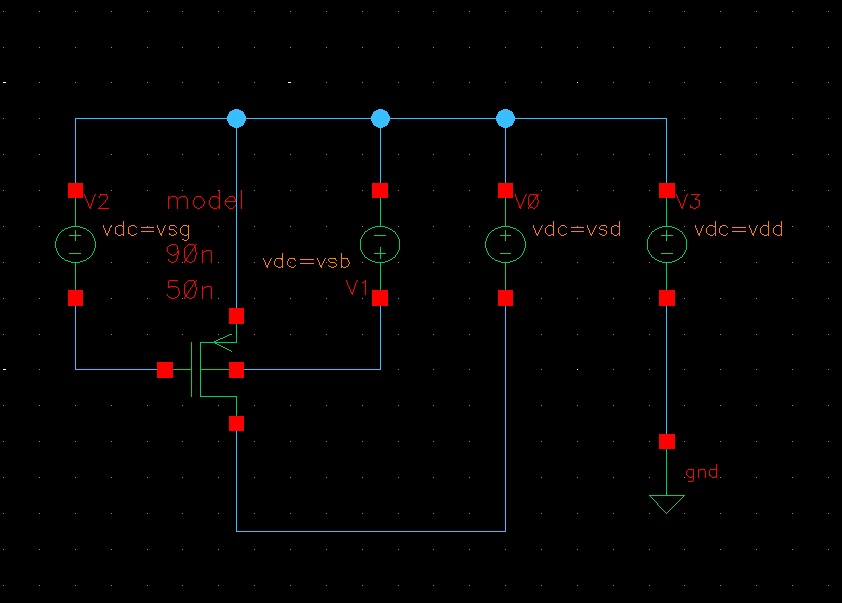
\includegraphics[width = 0.6\linewidth]{sections/pic/EX3_PMOS_schematic.png}
	\caption{Testbench PMOS\_VTG for experiment 3.}
	\label{f_ex3PMOS-schematic}
\end{figure}

\itemmini{Draw curves $I_{D}$ vs $V_{GS}$ @ $V_{DS} = 1V$, $V_{SB} = [0.1, 0.55, 0.9] V$, and sweeping $V_{GS} = [0, 1]V$ with step $10mV$.}

\begin{figure}[H]
	\centering
	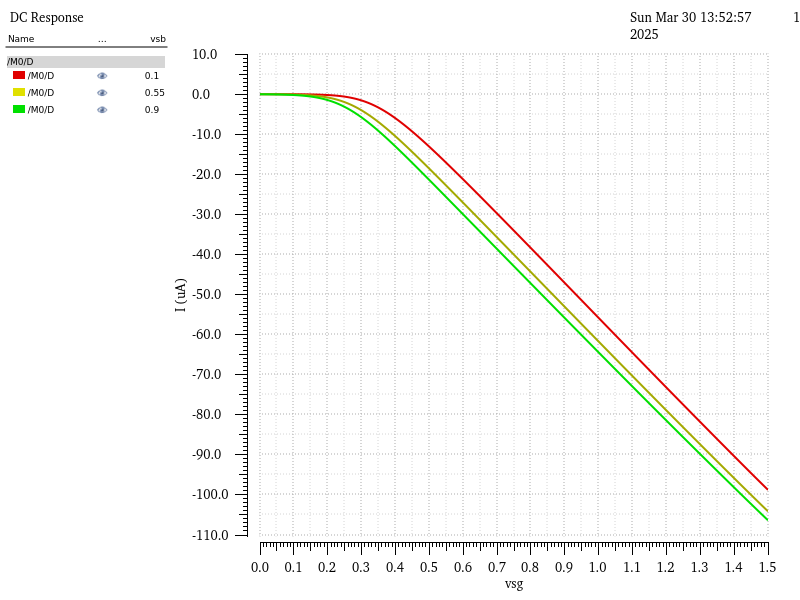
\includegraphics[width=.6\linewidth]{sections/pic/EX3_PMOS_Id&Vgs(Vds=0_1)(w)(l).png}
	\caption{$I_{D}$ vs $V_{GS}$ @ $V_{DS} = 1V$, $V_{SB} = [0.1, 0.55, 0.9] V$, and sweeping $V_{GS} = [0, 1]V$ with step $10mV$.}
	\label{f_EX3_PMOS_Id&Vgs(Vds=0_1)(w)(l)}
\end{figure}

\itemmini{Draw curves $I_{D}$ vs $V_{DS}$ @ $V_{GS} = 1V$, $V_{SB} = [0.1, 0.55, 0.9] V$, and sweeping $V_{DS} = [0, 1]V$ with step $10mV$.}

\begin{figure}[H]
	\centering
	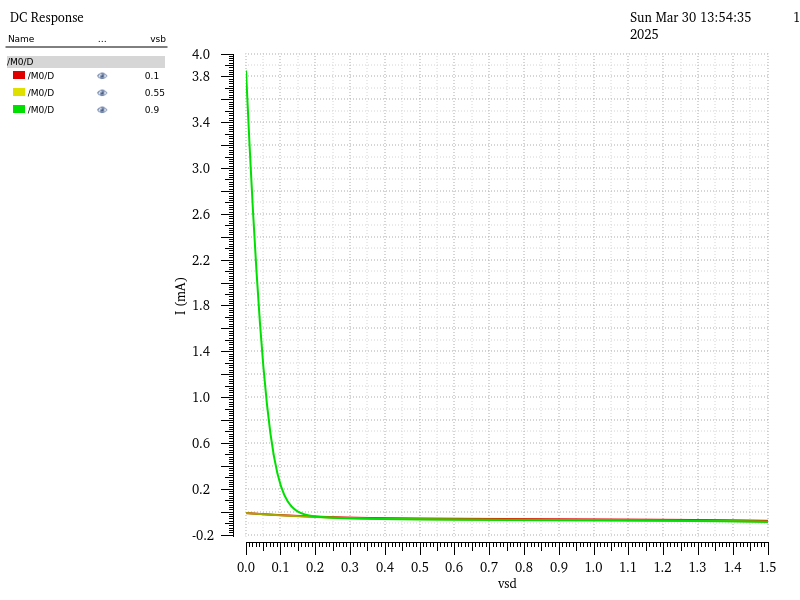
\includegraphics[width=.6\linewidth]{sections/pic/EX3_PMOS_Id&Vds(Vgs=0_1)(w)(l).png}
	\caption{$I_{D}$ vs $V_{DS}$ @ $V_{GS} = 1V$, $V_{SB} = [0.1, 0.55, 0.9] V$, and sweeping $V_{DS} = [0, 1]V$ with step $10mV$.}
	\label{f_EX3_PMOS_Id&Vds(Vgs=0_1)(w)(l)}
\end{figure}


\subsubsection{Measure $\lambda$}
\textbf{Note:} Take points in the saturation region.\\

Draw the curves for $I_{D}$ vs $V_{DS} = [0, 1.5](V)$ with a step of $10mV$, for two values of $V_{GS} = \{0.5, 0.75\}$.\\

\itemmini{For the PMOS transistor with $(W/L) = (90n/50n)$.}

\begin{figure}[H]
	\centering
	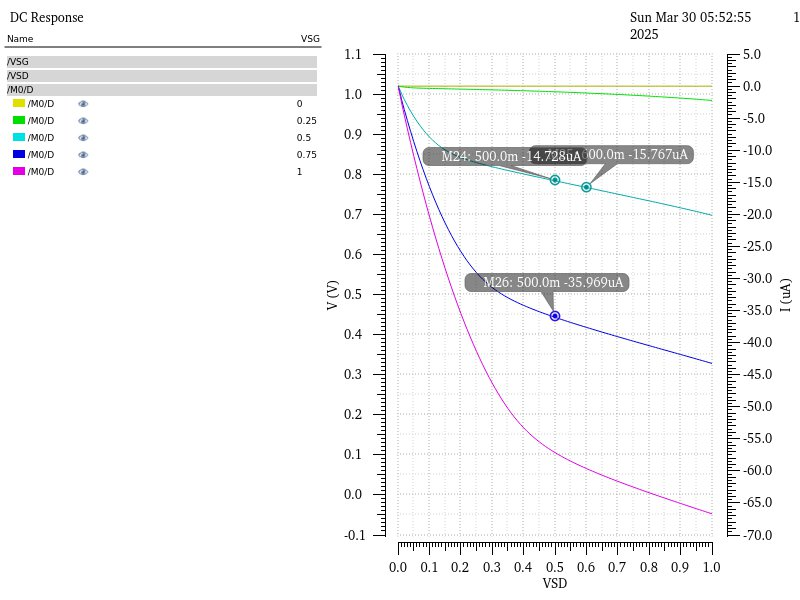
\includegraphics[width=0.6\linewidth]{sections/pic/EX3_PMOS_lambda_(w_l)(90_50).png}
	\caption{$I_{DS}$ vs $V_{DS}$ with step $10mV$ for value of $V_{GS} = 0.5V$ and $(W/L) = (90n/50n)$}
	\label{f_EX3_PMOS_lambda_(w_l)(90_50)}
\end{figure}

\[ \lambda = \dfrac{I_{D2} - I_{D1}}{I_{D1} V_{DS2} - I_{D2} V_{DS1}} \]

With $V_{GS} = 0.5$, we have:

\[ \lambda = \dfrac{I_{D2} - I_{D1}}{I_{D1} V_{DS2} - I_{D2} V_{DS1}} = \dfrac{(-15.77 - -14.73)\times 10^{-6}}{-15.77\times 10^{-6}\times 0.5 - -14.73 \times 10^{-6} \times 0.4 }  = 1.09\]

%Với $V_{GS} = 0.75$ ta có:
%
%\[ \lambda = \dfrac{I_{D2} - I_{D1}}{I_{D1} V_{DS2} - I_{D2} V_{DS1}} = \dfrac{(59.73 - -35.97)\times 10^{-6}}{57.28\times 10^{-6}\times 0.5 - 59.73 \times 10^{-6} \times 0.4 }  = 0.52\]

%Ta thấy $\lambda(0.5)> \lambda(0.75)$. Điều này có nghĩa là khi $V_{GS}$ thấp, độ ổn định của $I_{DS}$ trong vùng bão hòa kém hơn.\\ 

\itemmini{For the PMOS transistor with $(W/L) = (120n/60n)$.}

\begin{figure}[H]
	\centering
	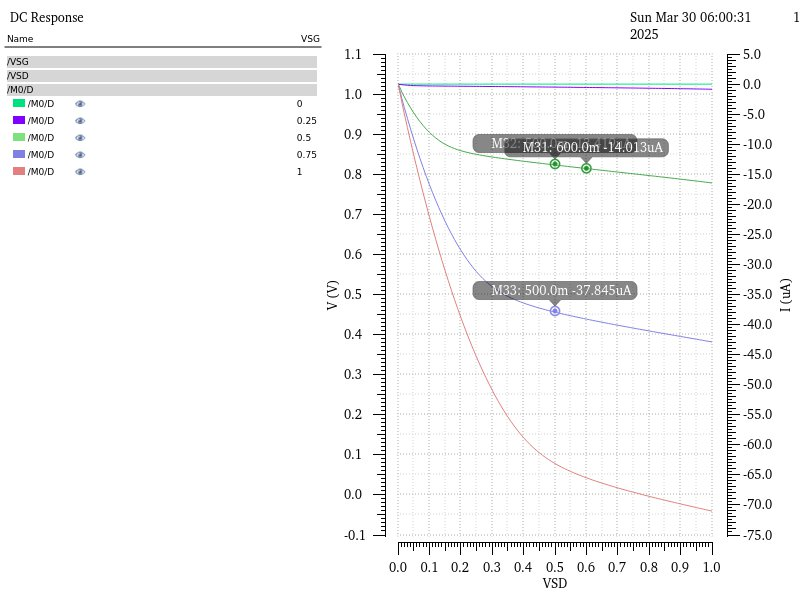
\includegraphics[width=.6\linewidth]{sections/pic/EX3_PMOS_lambda_(w_l)(120_90)(vgs_0_5).png}
	\caption{$I_{DS}$ vs $V_{DS}$ with step $10mV$  for value of $V_{GS} = 0.5$ and $(W/L) = (120n/60n)$}
	\label{f_EX3_PMOS_lambda_(w_l)(120_90)(vgs_0_5)}
\end{figure}

With $V_{GS} = 0.5$, we have:

\[ \lambda = \dfrac{I_{D2} - I_{D1}}{I_{D1} V_{DS2} - I_{D2} V_{DS1}} = \dfrac{(-14.01 - -13.41)\times 10^{-6}}{-13.41\times 10^{-6}\times 0.5 - -14.01 \times 10^{-6} \times 0.4 }  = 0.576 \]

%Vậy khi PMOS có công nghệ càng nhỏ thì $\lambda$ càng tăng. Lý do là khi $L$ giảm, hiệu ứng \textit{Chiều dài kênh ngắn (SCE - Short Channel Effect)} trở nên rõ nệt hơn, làm tăng sự phụ thuộc của $I_{DS}$ và $V_{DS}$. Điều này khiến cho hệ số $\lambda$ tăng lên, nghĩa là $I_{DS}$ kém ổn định hơn.

\subsubsection{Measure $V_{Th0}$}
\[ V_{Th} = \dfrac{V_{GS1} - V_{GS2}\sqrt{\dfrac{I_{DS1}}{I_{DS2}}}}{1 - \sqrt{\dfrac{I_{DS1}}{I_{DS2}}}} \]

\itemmini{For the PMOS transistor with $(W/L) = (90n/50n)$.}

\begin{figure}[H]
	\centering
	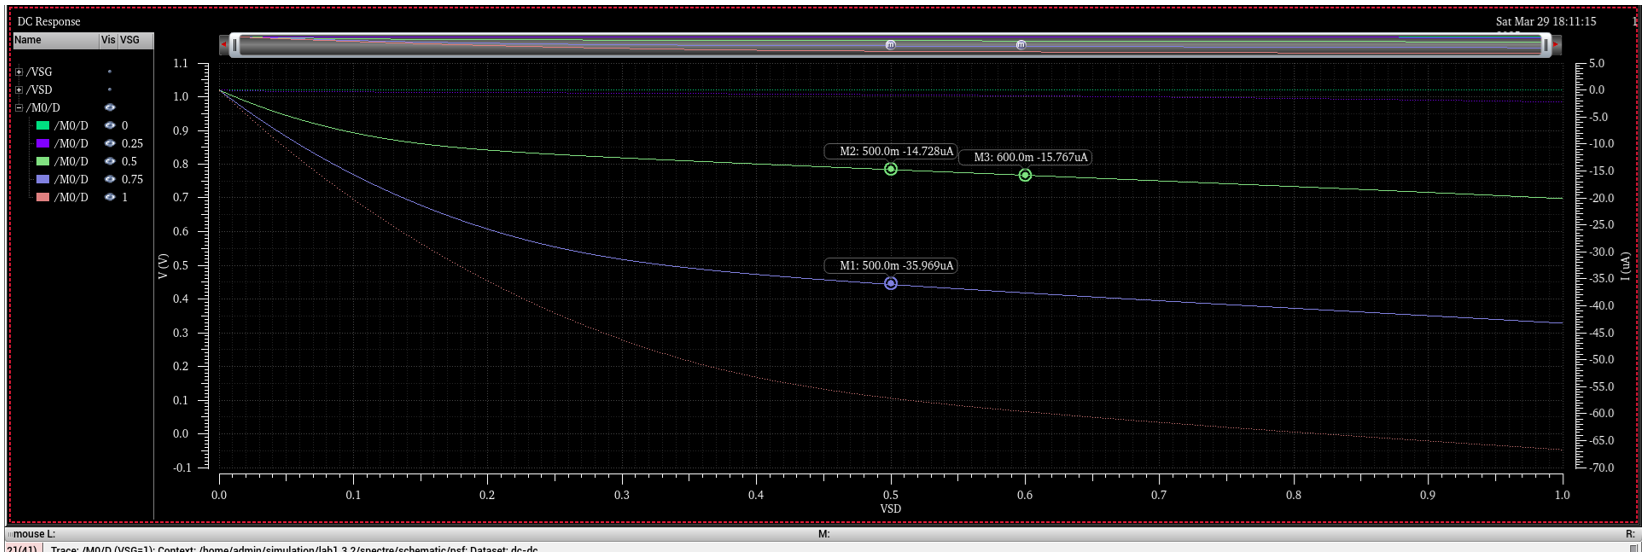
\includegraphics[width=.6\linewidth]{sections/pic/EX3_PMOS_vth0_(w_l)(90_50).png}
	\caption{$I_{DS}$ vs $V_{DS}$ with step $10mV$ for $(W/L) = (90n/50n)$}
	\label{f_EX3_PMOS_vth0_(w_l)(90_50)}
\end{figure}

\[ V_{Th0} = \dfrac{V_{GS1} - V_{GS2}\sqrt{\dfrac{I_{DS1}}{I_{DS2}}}}{1 - \sqrt{\dfrac{I_{DS1}}{I_{DS2}}}} = \dfrac{0.75 - 0.5\times \sqrt{\dfrac{-35.97\times 10^{-6}}{-14.73\times 10^{-6}}}}{1 - \sqrt{\dfrac{-35.79\times 10^{-6}}{-14.73\times 10^{-6}}}} = 0.056(V)\]

\itemmini{For the PMOS transistor with $(W/L) = (120n/60n)$.}

\begin{figure}[H]
	\centering
	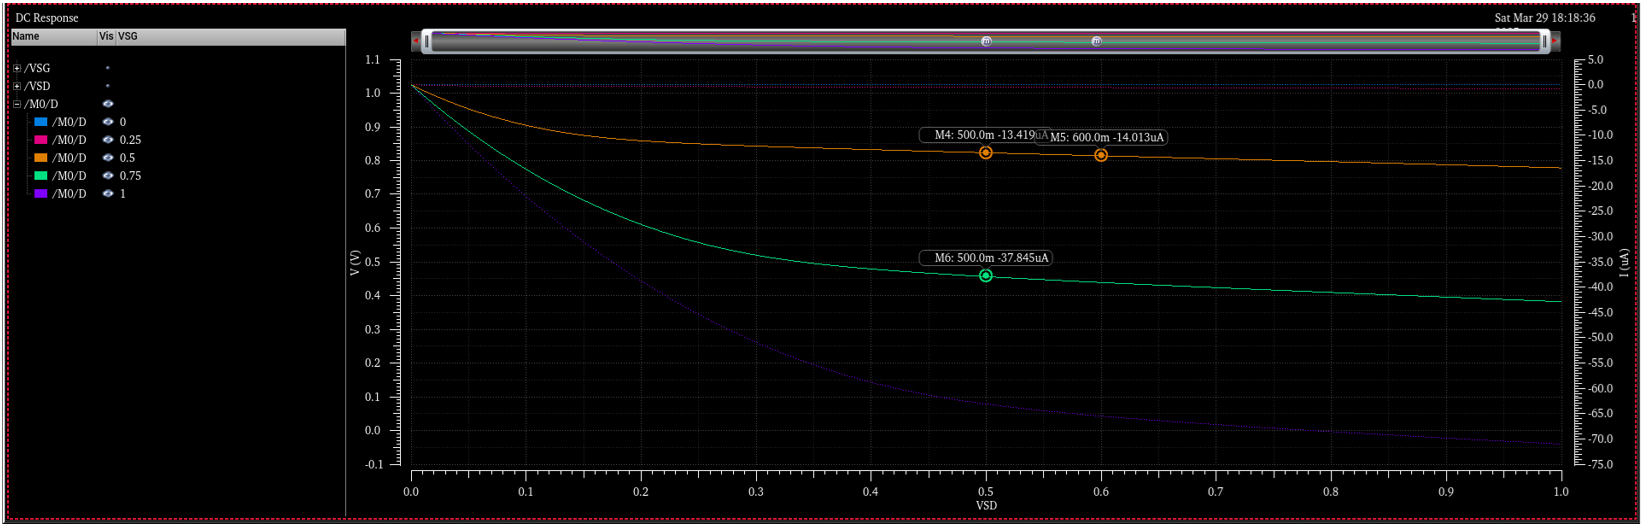
\includegraphics[width=.6\linewidth]{sections/pic/EX3_PMOS_vth0_(w_l)(120_60).png}
	\caption{$I_{DS}$ vs $V_{DS}$ with step $10mV$ for $(W/L) = (120n/60n)$}
	\label{f_EX3_PMOS_vth0_(w_l)(120_60)}
\end{figure}

\[ V_{Th0} = \dfrac{V_{GS1} - V_{GS2}\sqrt{\dfrac{I_{DS1}}{I_{DS2}}}}{1 - \sqrt{\dfrac{I_{DS1}}{I_{DS2}}}} = \dfrac{0.75 - 0.5\times \sqrt{\dfrac{-37.85\times 10^{-6}}{-13.42\times 10^{-6}}}}{1 - \sqrt{\dfrac{-37.85\times 10^{-6}}{-13.42\times 10^{-6}}}} = 0.132(V)\] 


%KHi tỷ lệ $W/L$ thay đổi, $VTH$ có thể bị ảnh hưởng do hiệu ứng \textit{Chiều dài kênh ngắn (SCE)}.
%
%Khi $L$ giảm (trong trường hợp PMOS $90n/50n$), $VTH$ có xu hướng giảm do hiệu ứng kéo rào thế xuống (DIBL - Drain-Induced Barrier Lowering).
%
%Khi $L$ lớn hơn (trong trường hợp PMOS $120n/60n$), $VTH$ cao hơn vì hiệu ứng chiều dài kênh ngắn ít rõ rệt hơn.

\subsubsection{Measure $\gamma$}

\itemmini{For the PMOS transistor with $(W/L) = (90n/50n)$ và $V_{BS} = 0.5$.}

\begin{figure}[H]
	\centering
	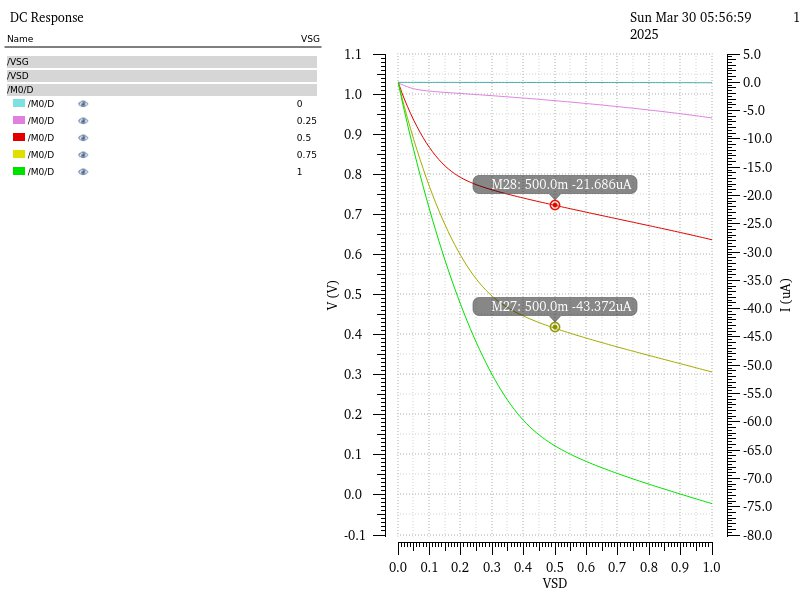
\includegraphics[width=.6\linewidth]{sections/pic/EX3_PMOS_gamma_(w_l)(90_50).png}
	\caption{$I_{DS}$ vs. $V_{DS}$ with a step of $10,\text{mV}$ for $(W/L) = (90n/50n)$}
	\label{f_EX3_PMOS_gamma_(w_l)(90_50)}
\end{figure}

\[ V_{Th} = \dfrac{V_{GS1} - V_{GS2}\sqrt{\dfrac{I_{DS1}}{I_{DS2}}}}{1 - \sqrt{\dfrac{I_{DS1}}{I_{DS2}}}} = \dfrac{0.75 - 0.5\times \sqrt{\dfrac{-43.37\times 10^{-6}}{-21.68\times 10^{-6}}}}{1 - \sqrt{\dfrac{-43.37\times 10^{-6}}{-21.68\times 10^{-6}}}} = -0.103(V)\] 


We have, $2\phi F = 0.7 \gamma$:

\[ \gamma = \dfrac{V_{Th} - V_{Th0}}{\sqrt{|2\phi_{F}| + |V_{BS} } - \sqrt{|2\phi_{F}}} = \dfrac{-0.103 - 0.056}{\sqrt{0.7 + 0.5} - \sqrt{0.7}} =-0.182 \]

%Vậy ta có thể kết luận khi $\gamma$ tăng khiến $V_{Th}$ tăng mạnh hơn khi $V_{BS}$ tăng.\\
When $V_{BS}$ increases, the $V_{Th}$ of PMOS typically rises, but the extent of this change depends on the sign of $\gamma$ and the fabrication technology.\\

\itemmini{For the PMOS transistor with $(W/L) = (120n/60n)$ and $V_{BS} = 0.5$.}

\begin{figure}[H]
	\centering
	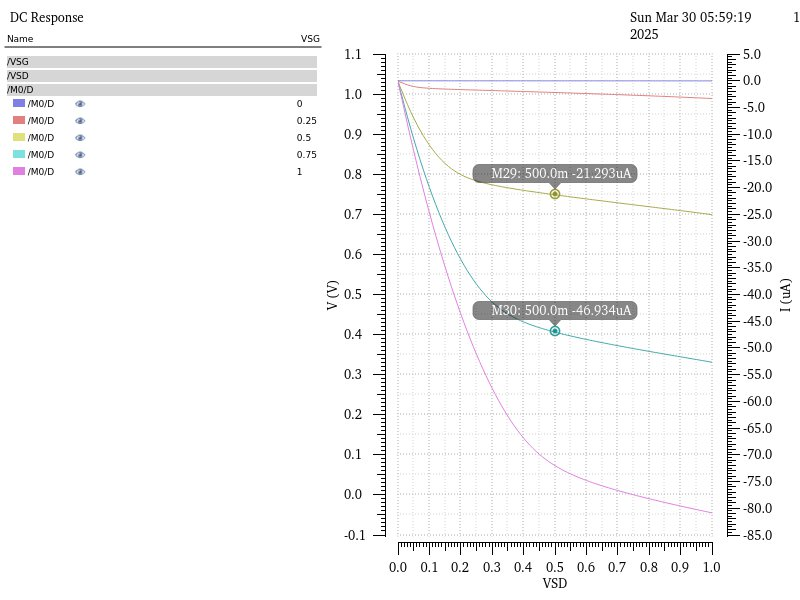
\includegraphics[width=.6\linewidth]{sections/pic/EX3_PMOS_gamma_(w_l)(120_60).png}
	\caption{$I_{DS}$ vs $V_{DS}$ with step $10mV$ với $(W/L) = (120n/60n)$}
	\label{f_EX3_PMOS_gamma_(w_l)(120_60)}
\end{figure}

\[ V_{Th} = \dfrac{V_{GS1} - V_{GS2}\sqrt{\dfrac{I_{DS1}}{I_{DS2}}}}{1 - \sqrt{\dfrac{I_{DS1}}{I_{DS2}}}} = \dfrac{0.75 - 0.5\times \sqrt{\dfrac{-46.93\times 10^{-6}}{-21.29\times 10^{-6}}}}{1 - \sqrt{\dfrac{-46.93\times 10^{-6}}{-21.29\times 10^{-6}}}} = -0.016(V)\] 

\[ \gamma = \dfrac{V_{Th} - V_{Th0}}{\sqrt{|2\phi_{F}| + |V_{BS} } - \sqrt{|2\phi_{F}}} = \dfrac{-0.016 - 0.132}{\sqrt{0.7 + 0.5} - \sqrt{0.7}} = -0.572 \]

\subsubsection{Measure $k_p$}

\itemmini{For the PMOS transistor with $(W/L) = (90n/50n)$}

\[ k_p = \dfrac{2I_{D}}{\dfrac{L}{W} (V_{GS} - V_{Th0})^{2} (1 + \lambda V_{DS})} = \dfrac{2\times -14.73 \times 10^{-6}}{\dfrac{50n}{90n} (0.5 - 0.056)^{2} (1 + 0.5 \times 1.09)} = -174 \times 10^{-6}\]

\itemmini{For the PMOS transistor with $(W/L) = (120n/60n)$}

\[ k_p = \dfrac{2I_{D}}{\dfrac{L}{W} (V_{GS} - V_{Th0})^{2} (1 + \lambda V_{DS})} = \dfrac{2\times -13.42 \times 10^{-6}}{\dfrac{60n}{120n} (0.5 - 0.132)^{2} (1 + 0.576 \times 0.5)} = -308 \times 10^{-6}\]



	\newpage
\section{Layout design for MOS transistor}

\subsection{NMOS}
\itemmini{Design the layout for an NMOS\_VTL (120n/60n), ensuring compliance with Design Rule Check (DRC). Verify the corresponding throught Layout Versus Schematic (LVS) confirmation.}\\ 

\itemmini{Schematic}\\

\begin{figure}[H]
	\centering
	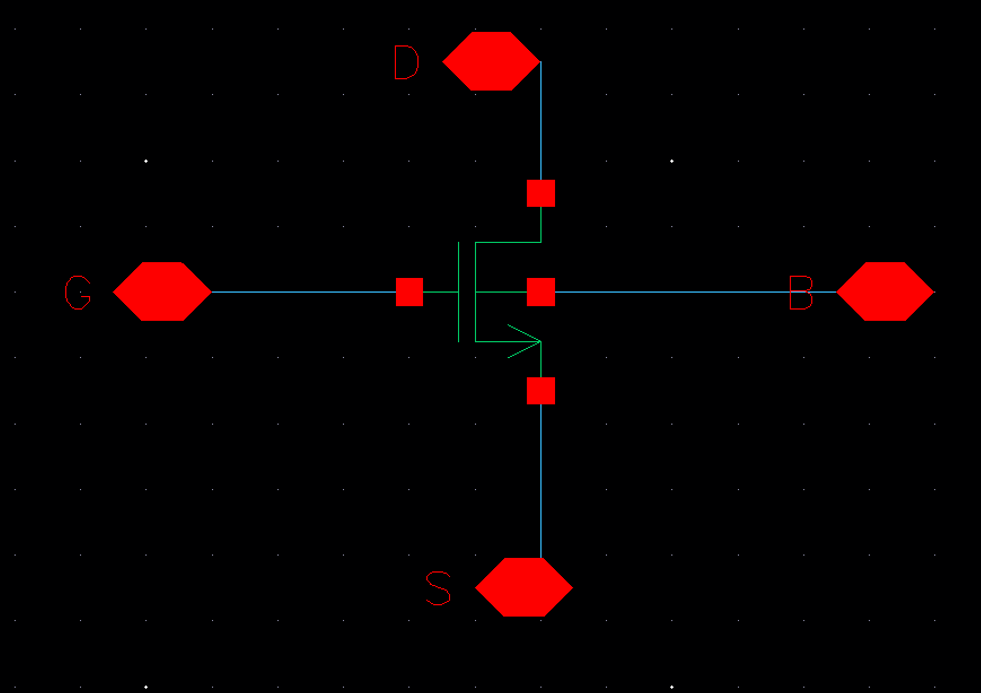
\includegraphics[width=.7\linewidth]{sections/pic/EX4_NMOS_schematic.png}
	\caption{Schematric NMOS ($(W/L) = (120n/90n)$).}
	\label{f_EX4_NMOS_schematic}
\end{figure}

\itemmini{Layout}\\

\begin{enumerate}[leftmargin=*, label = Step \arabic*:]
	\item Add \textit{n-active} layer define the active region dimensions based on the schematic parameters.
	\item Add Poly layer following the Rule ($\text{Contact} \geq 65nm$ and $\text{Poly} \geq 50nm$).
%	\item Thêm lớp \textbf{pimplant|drw} và \textbf{nimplant|drw} phủ theo kích thước Active.
	\item  Create drain, source, and bulk connections.
	\item Draw \textit{p-well} ensure compliance with design rules
	\item Cover with Metal1 layer.
	\begin{figure}[H]
		\centering
		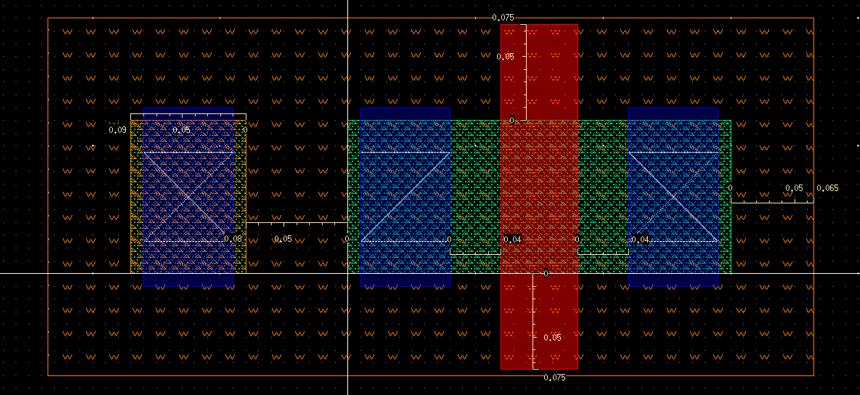
\includegraphics[width=.7\linewidth]{sections/pic/EX4_NMOS_metal.png}
		\label{f_EX4_NMOS_metal}
	\end{figure}
	\item Design the Gate structure includes: Contact, Metal1, and Poly.\\
	(\textit{Note: Gate Poly must adhere to distinct width/spacing rules (different from Active-to-Poly connections).}\\
	\begin{figure}[H]
		\centering
		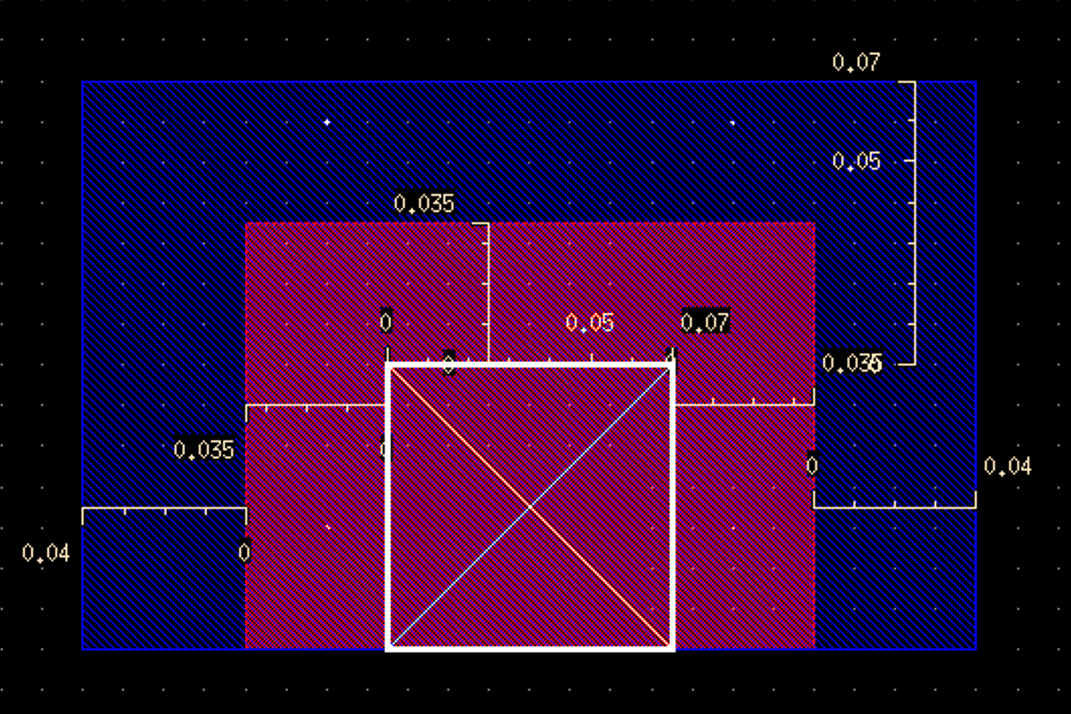
\includegraphics[width=.7\linewidth]{sections/pic/EX4_NMOS_gate.png}
		\label{f_EX4_NMOS_gate}		
	\end{figure}
	\item Add Metal2 and Vias.
	\begin{figure}[H]
		\centering
		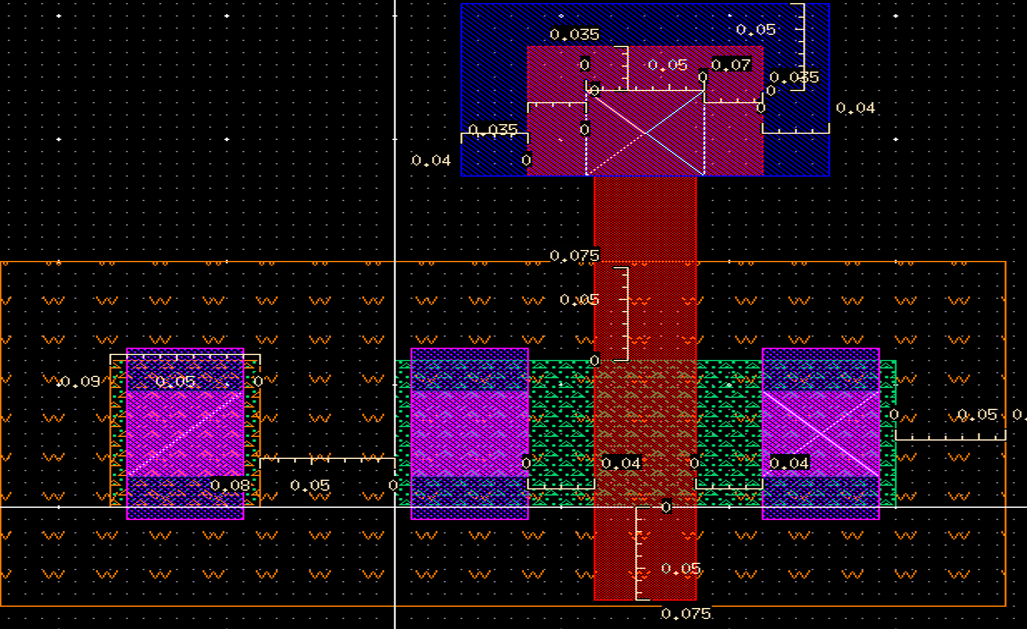
\includegraphics[width=.7\linewidth]{sections/pic/EX4_NMOS_metal2_vias.png}
		\label{f_EX4_NMOS_metal2_vias}
	\end{figure}
	\item Schematic-Layout Verification.
	\begin{figure}[H]
		\centering
		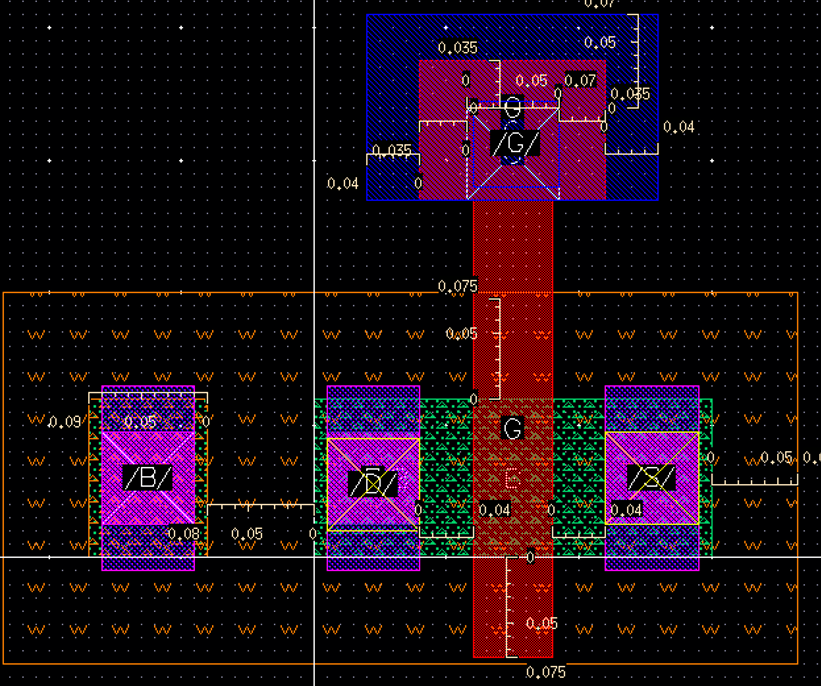
\includegraphics[width=.7\linewidth]{sections/pic/EX4_NMOS_layout_schematic.png}
		\label{f_EX4_NMOS_layout_schematic}
	\end{figure}
\end{enumerate}

\itemmini{Check DRC}\\

\begin{figure}[H]
	\centering
	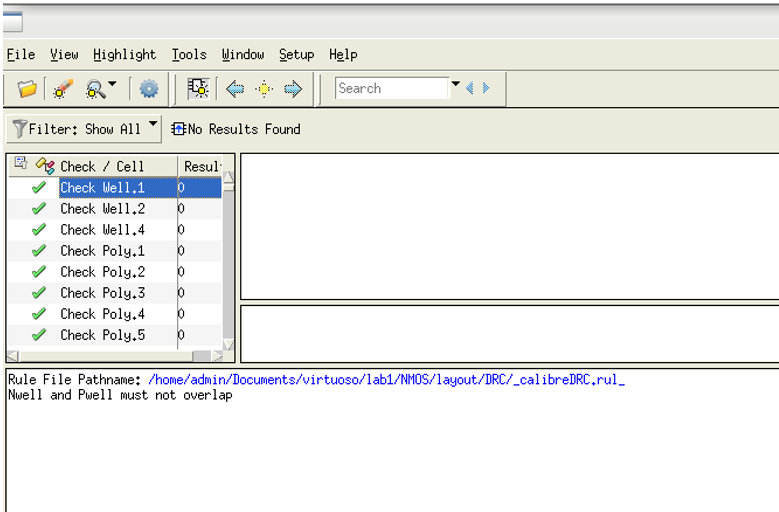
\includegraphics[width=.7\linewidth]{sections/pic/EX4_NMOS_DRC.png}
	\label{f_EX4_NMOS_DRC}
\end{figure}

\itemmini{Check LVS} \\

\begin{figure}[H]
	\centering
	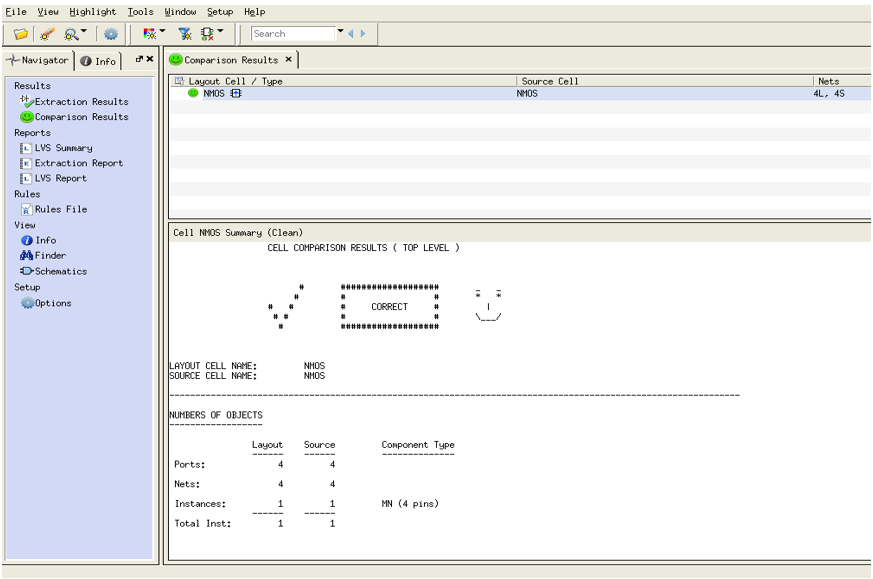
\includegraphics[width=.7\linewidth]{sections/pic/EX4_NMOS_LVS.png}
	\label{f_EX4_NMOS_LVS}
\end{figure}

\subsection{PMOS}
\itemmini{Design the layout for an PMOS\_VTL (50n/40n), ensuring compliance with Design Rule Check (DRC). Verify the corresponding throught Layout Versus Schematic (LVS) confirmation.}

\itemmini{Schematic}\\

\begin{figure}[H]
	\centering
	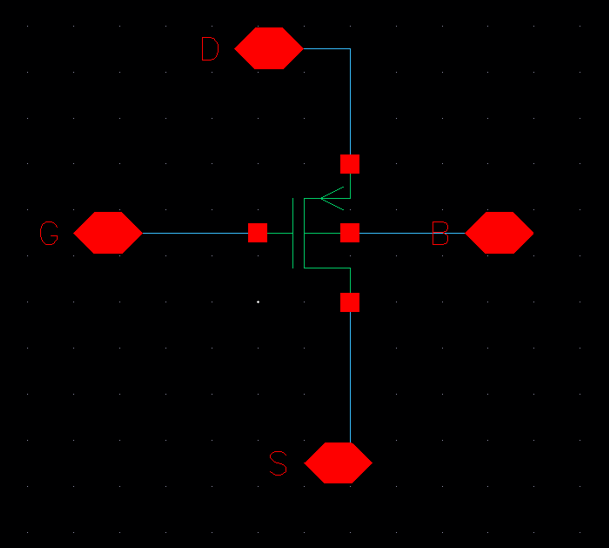
\includegraphics[width=.7\linewidth]{sections/pic/EX4_PMOS_schematic.png}
	\caption{Schematric PMOS ($(W/L) = (120n/90n)$).}
	\label{f_EX4_PMOS_schematic}
\end{figure}

\itemmini{Layout}\\

\begin{enumerate}[leftmargin=*, label = Step \arabic*:]
	\item Add \textit{n-active} layer define the active region dimensions based on the schematic parameters.
	\item Add Poly layer following the Rule ($\text{Contact} \geq 65nm$ and $\text{Poly} \geq 50nm$).
	%	\item Thêm lớp \textbf{pimplant|drw} và \textbf{nimplant|drw} phủ theo kích thước Active.
	\item  Create drain, source, and bulk connections.
	\item Draw \textit{p-well} ensure compliance with design rules
	\item Cover with Metal1 layer.
	\begin{figure}[H]
		\centering
		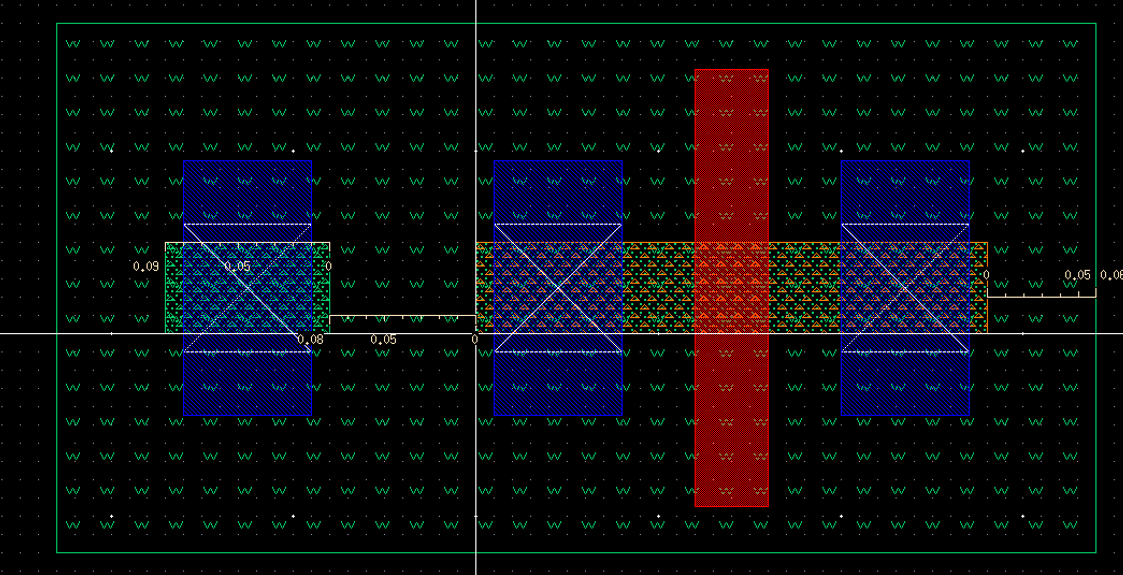
\includegraphics[width=.7\linewidth]{sections/pic/EX4_PMOS_metal.png}
		\label{f_EX4_PMOS_metal}
	\end{figure}
		\item Design the Gate structure includes: Contact, Metal1, and Poly.\\
	(\textit{Note: Gate Poly must adhere to distinct width/spacing rules (different from Active-to-Poly connections).}\\
	\begin{figure}[H]
		\centering
		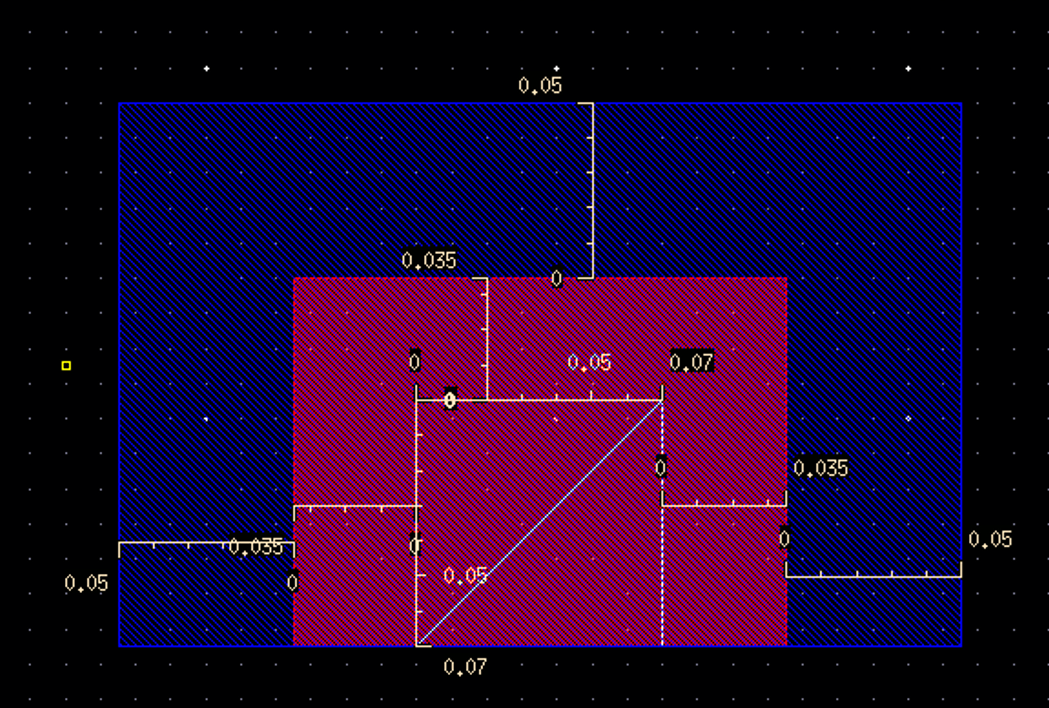
\includegraphics[width=.7\linewidth]{sections/pic/EX4_PMOS_gate.png}
		\label{f_EX4_PMOS_gate}		
	\end{figure}
	\item Add Metal2 and Vias.
	\begin{figure}[H]
		\centering
		\includegraphics[width=.7\linewidth]{sections/pic/EX4_PMOS_metal2_vias.png}
		\label{f_EX4_PMOS_metal2_vias}
	\end{figure}
	\item Schematic-Layout Verification.
	\begin{figure}[H]
		\centering
		\includegraphics[width=.7\linewidth]{sections/pic/EX4_PMOS_layout_schematic.png}
		\label{f_EX4_PMOS_layout_schematic}
	\end{figure}
\end{enumerate}

\itemmini{Check DRC}\\

\begin{figure}[H]
	\centering
	\includegraphics[width=.7\linewidth]{sections/pic/EX4_PMOS_DRC.png}
	\label{f_EX4_PMOS_DRC}
\end{figure}

The error is due to Poly requiring a minimum of $50n$ but the requirement is set at $40n$.

\begin{figure}[H]
	\centering
	\includegraphics[width=.7\linewidth]{sections/pic/EX4_PMOS_DRC_minpoly_50.png}
	\label{f_EX4_PMOS_DRC_minpoly_50}
\end{figure}

The error occurs because the \textit{Active} region requires a minimum width of \$90n\$ but is set to \$50n\$. The small \textit{Active} region prevents the \textit{Contact} from fully covering it, resulting in the error.

\begin{figure}[H]
	\centering
	\includegraphics[width=.7\linewidth]{sections/pic/EX4_PMOS_DRC_minactive_90.png}
	\label{f_EX4_PMOS_DRC_minactive}
\end{figure}

\itemmini{Check LVS}\\

\begin{figure}[H]
	\centering
	\includegraphics[width=.7\linewidth]{sections/pic/EX4_PMOS_LVS.png}
	\label{f_EX4_PMOS_LVS}
\end{figure}
\end{document}